%%
%% This is file `sample-manuscript.tex',
%% generated with the docstrip utility.
%%
%% The original source files were:
%%
%% samples.dtx  (with options: `all,proceedings,bibtex,manuscript')
%% 
%% IMPORTANT NOTICE:
%% 
%% For the copyright see the source file.
%% 
%% Any modified versions of this file must be renamed
%% with new filenames distinct from sample-manuscript.tex.
%% 
%% For distribution of the original source see the terms
%% for copying and modification in the file samples.dtx.
%% 
%% This generated file may be distributed as long as the
%% original source files, as listed above, are part of the
%% same distribution. (The sources need not necessarily be
%% in the same archive or directory.)
%%
%%
%% Commands for TeXCount
%TC:macro \cite [option:text,text]
%TC:macro \citep [option:text,text]
%TC:macro \citet [option:text,text]
%TC:envir table 0 1
%TC:envir table* 0 1
%TC:envir tabular [ignore] word
%TC:envir displaymath 0 word
%TC:envir math 0 word
%TC:envir comment 0 0
%%
%%
%% The first command in your LaTeX source must be the \documentclass
%% command.
%%
%% For submission and review of your manuscript please change the
%% command to \documentclass[manuscript, screen, review]{acmart}.
%%
%% When submitting camera ready or to TAPS, please change the command
%% to \documentclass[sigconf]{acmart} or whichever template is required
%% for your publication.
%%
%%
% \documentclass[manuscript,screen,review]{acmart}
%\documentclass[manuscript]{acmart}  % anonymous
\documentclass[sigconf]{acmart}


%%
%% \BibTeX command to typeset BibTeX logo in the docs
\AtBeginDocument{%
  \providecommand\BibTeX{{%
    Bib\TeX}}}

%% Rights management information.  This information is sent to you
%% when you complete the rights form.  These commands have SAMPLE
%% values in them; it is your responsibility as an author to replace
%% the commands and values with those provided to you when you
%% complete the rights form.


% copy from email
\copyrightyear{2025} 
\acmYear{2025} 
\setcopyright{cc}
\setcctype{by}
\acmConference[CHI '25]{CHI Conference on Human Factors in Computing Systems}{April 26-May 1, 2025}{Yokohama, Japan}
\acmBooktitle{CHI Conference on Human Factors in Computing Systems (CHI '25), April 26-May 1, 2025, Yokohama, Japan}
\acmDOI{10.1145/3706598.3713589}
\acmISBN{979-8-4007-1394-1/25/04}

% below are the original


% \setcopyright{acmlicensed}
% \copyrightyear{2018}
% \acmYear{2018}
% \acmDOI{XXXXXXX.XXXXXXX}

%% These commands are for a PROCEEDINGS abstract or paper.
% \acmConference[Conference acronym 'XX]{Make sure to enter the correct
%   conference title from your rights confirmation emai}{June 03--05,
%   2018}{Woodstock, NY}
%%
%%  Uncomment \acmBooktitle if the title of the proceedings is different
%%  from ``Proceedings of ...''!
%%
%%\acmBooktitle{Woodstock '18: ACM Symposium on Neural Gaze Detection,
%%  June 03--05, 2018, Woodstock, NY}
% \acmISBN{978-1-4503-XXXX-X/18/06}


%%
%% Submission ID.
%% Use this when submitting an article to a sponsored event. You'll
%% receive a unique submission ID from the organizers
%% of the event, and this ID should be used as the parameter to this command.
%%\acmSubmissionID{123-A56-BU3}

%%
%% For managing citations, it is recommended to use bibliography
%% files in BibTeX format.
%%
%% You can then either use BibTeX with the ACM-Reference-Format style,
%% or BibLaTeX with the acmnumeric or acmauthoryear sytles, that include
%% support for advanced citation of software artefact from the
%% biblatex-software package, also separately available on CTAN.
%%
%% Look at the sample-*-biblatex.tex files for templates showcasing
%% the biblatex styles.
%%

%%
%% The majority of ACM publications use numbered citations and
%% references.  The command \citestyle{authoryear} switches to the
%% "author year" style.
%%
%% If you are preparing content for an event
%% sponsored by ACM SIGGRAPH, you must use the "author year" style of
%% citations and references.
%% Uncommenting
%% the next command will enable that style.
%%\citestyle{acmauthoryear}



%%%%%%%%%%%%%%%%%%%%%%%%%%%%%%%%%%%%%%%%%%%%%%%%%%%%%%%%%%%%%%%%%%
% CUSTOM COMMANDS AND PACKAGES
%%%%%%%%%%%%%%%%%%%%%%%%%%%%%%%%%%%%%%%%%%%%%%%%%%%%%%%%%%%%%%%%%%
\let\comment\undefined%added to fix error
% \PassOptionsToPackage{normalem}{ulem}%added to fix error
% \usepackage{changes}


%\let\uline\relax
\let\uuline\relax
\let\uwave\relax
\let\sout\relax
\let\xout\relax
\let\dotuline\relax
\let\dashuline\relax
\let\dashuline\relax
\let\ULdepth\relax
\let\ULset\relax


\usepackage{acmart-taps}
\usepackage{xcolor}
\usepackage{tabularray}
\usepackage{subcaption}
\usepackage{enumitem}
\usepackage{booktabs}   
\usepackage{array}      
\usepackage{arydshln}   
\usepackage{caption}   
\usepackage{color}

% \usepackage[margin=1in]{geometry}

%\newcommand{\todo}[1]{\textcolor{red}{[*** #1 ***]}}
% black blue


%%%%%%%%%%%%%%%%%%%%%%%%%%%%%%%%%%%%%%%%%%%%%%%%%%%%%%%%%%%%%%%%%%


\sloppy
%%
%% end of the preamble, start of the body of the document source.
\begin{document}

%%
%% The "title" command has an optional parameter,
%% allowing the author to define a "short title" to be used in page headers.
% \title{TutorUp: A Scenario-Based Learning Environment to Facilitate the Adoption of Effective Engagement Strategies in Remote Tutoring}
\title[TutorUp: Training Tutors to Address Engagement Challenges in Online Learning]{TutorUp: What If Your Students Were Simulated? Training Tutors to Address Engagement Challenges in Online Learning}
% %%
% %% The "author" command and its associated commands are used to define
% %% the authors and their affiliations.
% %% Of note is the shared affiliation of the first two authors, and the
% %% "authornote" and "authornotemark" commands
% %% used to denote shared contribution to the research.
% \author{Ben Trovato}
% \authornote{Both authors contributed equally to this research.}
% \email{trovato@corporation.com}
% \orcid{1234-5678-9012}
% \author{G.K.M. Tobin}
% \authornotemark[1]
% \email{webmaster@marysville-ohio.com}
% \affiliation{%
%   \institution{Institute for Clarity in Documentation}
%   \city{Dublin}
%   \state{Ohio}
%   \country{USA}
% }

\author{Sitong Pan}
\affiliation{%
  \institution{Zhejiang University}
  \city{Hangzhou}
  \country{China}}
\email{pstong@zju.edu.cn}

\author{Robin Schmucker}
 \affiliation{%
 \institution{Carnegie Mellon University}
 \city{Pittsburgh}
 \state{PA}
 \country{USA}
}
\email{rschmuck@cs.cmu.edu}


\author{Bernardo Garcia Bulle Bueno}
\affiliation{%
\institution{Massachusetts Institute of Technology}
\city{Cambridge}
\state{MA}
\country{USA}}
\email{bernard0@mit.edu}


\author{Salome Aguilar Llanes}
\affiliation{%
\institution{Massachusetts Institute of Technology}
\city{Cambridge}
\state{MA}
\country{USA}}
\email{saloagui@mit.edu}

\author{Fernanda Albo Alarcón}
\affiliation{%
  % \institution{Jóvenes Ayudando a Niñas y Niños}
  \institution{Autonomous Technological Institute of Mexico}
  \city{Mexico City}
  \country{Mexico}}
\email{fer.albo.al@gmail.com}

 \author{Hangxiao Zhu}
\affiliation{%
   \institution{Texas A\&M University}
   \city{College Station}
   \state{TX}
   \country{USA}
   }
\email{hangxiao@tamu.edu}

 \author{Adam Teo}
\affiliation{%
   \institution{Texas A\&M University}
   \city{College Station}
   \state{TX}
   \country{USA}
   }
\email{adamt321@tamu.edu}

\author{Meng Xia}
\affiliation{%
   \institution{Texas A\&M University}
   \city{College Station}
   \state{TX}
   \country{USA}
   }
\email{mengxia@tamu.edu}


% %%
% %% By default, the full list of authors will be used in the page
% %% headers. Often, this list is too long, and will overlap
% %% other information printed in the page headers. This command allows
% %% the author to define a more concise list
% %% of authors' names for this purpose.
\renewcommand{\shortauthors}{Pan et al.}

%%
%% The abstract is a short summary of the work to be presented in the
%% article.
\begin{abstract}
%With the rise of online learning, many novice tutors become online teachers. However, many lack experience in facilitating student engagement during remote tutoring, and practicing with real students is costly and potentially harmful. In response, we introduce TutorUp, an LLMs-based system that enables tutors to practice engagement strategies with simulated students in different teaching scenarios. These scenarios mimic real world teaching settings and are based on a formative study, which included surveys and interviews (N=108) exploring student engagement issues in online learning. Particularly, to promote realistic simulations, we employ a prompting strategy that "tells the story" of online session dialogues. We further employ LLMs to provide immediate and asynchronous feedback by referencing user inputs and established teaching strategies derived from the literature. In a within-subject evaluation (N=16), participants rated our system significantly higher than the baseline across effectiveness and usability. Compared to the baseline system, TutorUp allows tutors to more effectively learn and apply strategies for engaging students. % 
% With the rise of online learning, many novice tutors become online teachers. However, many lack experience in facilitating student engagement in remote settings. In response, we introduce TutorUp, a Large Language Model (LLM)-based system that enables tutors to practice engagement strategies with simulated students in scenario-based training. These scenarios mimic real teaching situations based on a formative study (N=108), which included surveys and interviews exploring student engagement issues in online learning. To promote immersive simulations, we employ a prompting strategy that iteratively "tells the story" of online learning dialogues. Additionally, TutorUp provides immediate and asynchronous feedback by referencing user inputs and teaching strategies from the learning science literature. In a within-subject evaluation (N=16), participants rated TutorUp significantly higher than a baseline system across effectiveness and usability. Our findings suggest that TutorUp allows tutors to learn and apply strategies for engaging students more effectively, contributing to improved practices in online tutoring.
% Alternative version
With the rise of online learning, many novice tutors lack experience engaging students remotely. We introduce \textit{TutorUp}, a Large Language Model (LLM)-based system that enables novice tutors to practice engagement strategies with simulated students through scenario-based training. Based on a formative study involving two surveys ($N_1=86$, $N_2=102$) on student engagement challenges, we summarize scenarios that mimic real teaching situations. To enhance immersion and realism, we employ a prompting strategy that simulates dynamic online learning dialogues. \textit{TutorUp} provides immediate and asynchronous feedback by referencing tutor-students online session dialogues and evidence-based teaching strategies from learning science literature. In a within-subject evaluation ($N=16$), participants rated \textit{TutorUp} significantly higher than a baseline system without simulation capabilities regarding effectiveness and usability. Our findings suggest that \textit{TutorUp} provides novice tutors with more effective training to learn and apply teaching strategies to address online student engagement challenges. 
\end{abstract}
% helps tutors learn and apply strategies for more effective student engagement, contributing to improved practices in online tutoring.
%%
%% The code below is generated by the tool at http://dl.acm.org/ccs.cfm.
%% Please copy and paste the code instead of the example below.
%%

\begin{CCSXML}
<ccs2012>
   <concept>
       <concept_id>10003120.10003121.10011748</concept_id>
       <concept_desc>Human-centered computing~Empirical studies in HCI</concept_desc>
       <concept_significance>500</concept_significance>
       </concept>
   <concept>
       <concept_id>10010405.10010489</concept_id>
       <concept_desc>Applied computing~Education</concept_desc>
       <concept_significance>500</concept_significance>
       </concept>
 </ccs2012>
\end{CCSXML}

\ccsdesc[500]{Human-centered computing~Empirical studies in HCI}
\ccsdesc[500]{Applied computing~Education}


%%
%% Keywords. The author(s) should pick words that accurately describe
%% the work being presented. Separate the keywords with commas.
\keywords{Remote Tutoring, Tutor Training, Interactive Learning Environments, Conversational Agents, Large Language Models, Student Engagement}

%\received{20 February 2007}
%\received[revised]{12 March 2009}
%\received[accepted]{5 June 2009}

%%
%% This command processes the author and affiliation and title
%% information and builds the first part of the formatted document.
\maketitle
% \begin{abstract}  
Test time scaling is currently one of the most active research areas that shows promise after training time scaling has reached its limits.
Deep-thinking (DT) models are a class of recurrent models that can perform easy-to-hard generalization by assigning more compute to harder test samples.
However, due to their inability to determine the complexity of a test sample, DT models have to use a large amount of computation for both easy and hard test samples.
Excessive test time computation is wasteful and can cause the ``overthinking'' problem where more test time computation leads to worse results.
In this paper, we introduce a test time training method for determining the optimal amount of computation needed for each sample during test time.
We also propose Conv-LiGRU, a novel recurrent architecture for efficient and robust visual reasoning. 
Extensive experiments demonstrate that Conv-LiGRU is more stable than DT, effectively mitigates the ``overthinking'' phenomenon, and achieves superior accuracy.
\end{abstract}  


\section{Introduction}
\label{sec:introduction}
The business processes of organizations are experiencing ever-increasing complexity due to the large amount of data, high number of users, and high-tech devices involved \cite{martin2021pmopportunitieschallenges, beerepoot2023biggestbpmproblems}. This complexity may cause business processes to deviate from normal control flow due to unforeseen and disruptive anomalies \cite{adams2023proceddsriftdetection}. These control-flow anomalies manifest as unknown, skipped, and wrongly-ordered activities in the traces of event logs monitored from the execution of business processes \cite{ko2023adsystematicreview}. For the sake of clarity, let us consider an illustrative example of such anomalies. Figure \ref{FP_ANOMALIES} shows a so-called event log footprint, which captures the control flow relations of four activities of a hypothetical event log. In particular, this footprint captures the control-flow relations between activities \texttt{a}, \texttt{b}, \texttt{c} and \texttt{d}. These are the causal ($\rightarrow$) relation, concurrent ($\parallel$) relation, and other ($\#$) relations such as exclusivity or non-local dependency \cite{aalst2022pmhandbook}. In addition, on the right are six traces, of which five exhibit skipped, wrongly-ordered and unknown control-flow anomalies. For example, $\langle$\texttt{a b d}$\rangle$ has a skipped activity, which is \texttt{c}. Because of this skipped activity, the control-flow relation \texttt{b}$\,\#\,$\texttt{d} is violated, since \texttt{d} directly follows \texttt{b} in the anomalous trace.
\begin{figure}[!t]
\centering
\includegraphics[width=0.9\columnwidth]{images/FP_ANOMALIES.png}
\caption{An example event log footprint with six traces, of which five exhibit control-flow anomalies.}
\label{FP_ANOMALIES}
\end{figure}

\subsection{Control-flow anomaly detection}
Control-flow anomaly detection techniques aim to characterize the normal control flow from event logs and verify whether these deviations occur in new event logs \cite{ko2023adsystematicreview}. To develop control-flow anomaly detection techniques, \revision{process mining} has seen widespread adoption owing to process discovery and \revision{conformance checking}. On the one hand, process discovery is a set of algorithms that encode control-flow relations as a set of model elements and constraints according to a given modeling formalism \cite{aalst2022pmhandbook}; hereafter, we refer to the Petri net, a widespread modeling formalism. On the other hand, \revision{conformance checking} is an explainable set of algorithms that allows linking any deviations with the reference Petri net and providing the fitness measure, namely a measure of how much the Petri net fits the new event log \cite{aalst2022pmhandbook}. Many control-flow anomaly detection techniques based on \revision{conformance checking} (hereafter, \revision{conformance checking}-based techniques) use the fitness measure to determine whether an event log is anomalous \cite{bezerra2009pmad, bezerra2013adlogspais, myers2018icsadpm, pecchia2020applicationfailuresanalysispm}. 

The scientific literature also includes many \revision{conformance checking}-independent techniques for control-flow anomaly detection that combine specific types of trace encodings with machine/deep learning \cite{ko2023adsystematicreview, tavares2023pmtraceencoding}. Whereas these techniques are very effective, their explainability is challenging due to both the type of trace encoding employed and the machine/deep learning model used \cite{rawal2022trustworthyaiadvances,li2023explainablead}. Hence, in the following, we focus on the shortcomings of \revision{conformance checking}-based techniques to investigate whether it is possible to support the development of competitive control-flow anomaly detection techniques while maintaining the explainable nature of \revision{conformance checking}.
\begin{figure}[!t]
\centering
\includegraphics[width=\columnwidth]{images/HIGH_LEVEL_VIEW.png}
\caption{A high-level view of the proposed framework for combining \revision{process mining}-based feature extraction with dimensionality reduction for control-flow anomaly detection.}
\label{HIGH_LEVEL_VIEW}
\end{figure}

\subsection{Shortcomings of \revision{conformance checking}-based techniques}
Unfortunately, the detection effectiveness of \revision{conformance checking}-based techniques is affected by noisy data and low-quality Petri nets, which may be due to human errors in the modeling process or representational bias of process discovery algorithms \cite{bezerra2013adlogspais, pecchia2020applicationfailuresanalysispm, aalst2016pm}. Specifically, on the one hand, noisy data may introduce infrequent and deceptive control-flow relations that may result in inconsistent fitness measures, whereas, on the other hand, checking event logs against a low-quality Petri net could lead to an unreliable distribution of fitness measures. Nonetheless, such Petri nets can still be used as references to obtain insightful information for \revision{process mining}-based feature extraction, supporting the development of competitive and explainable \revision{conformance checking}-based techniques for control-flow anomaly detection despite the problems above. For example, a few works outline that token-based \revision{conformance checking} can be used for \revision{process mining}-based feature extraction to build tabular data and develop effective \revision{conformance checking}-based techniques for control-flow anomaly detection \cite{singh2022lapmsh, debenedictis2023dtadiiot}. However, to the best of our knowledge, the scientific literature lacks a structured proposal for \revision{process mining}-based feature extraction using the state-of-the-art \revision{conformance checking} variant, namely alignment-based \revision{conformance checking}.

\subsection{Contributions}
We propose a novel \revision{process mining}-based feature extraction approach with alignment-based \revision{conformance checking}. This variant aligns the deviating control flow with a reference Petri net; the resulting alignment can be inspected to extract additional statistics such as the number of times a given activity caused mismatches \cite{aalst2022pmhandbook}. We integrate this approach into a flexible and explainable framework for developing techniques for control-flow anomaly detection. The framework combines \revision{process mining}-based feature extraction and dimensionality reduction to handle high-dimensional feature sets, achieve detection effectiveness, and support explainability. Notably, in addition to our proposed \revision{process mining}-based feature extraction approach, the framework allows employing other approaches, enabling a fair comparison of multiple \revision{conformance checking}-based and \revision{conformance checking}-independent techniques for control-flow anomaly detection. Figure \ref{HIGH_LEVEL_VIEW} shows a high-level view of the framework. Business processes are monitored, and event logs obtained from the database of information systems. Subsequently, \revision{process mining}-based feature extraction is applied to these event logs and tabular data input to dimensionality reduction to identify control-flow anomalies. We apply several \revision{conformance checking}-based and \revision{conformance checking}-independent framework techniques to publicly available datasets, simulated data of a case study from railways, and real-world data of a case study from healthcare. We show that the framework techniques implementing our approach outperform the baseline \revision{conformance checking}-based techniques while maintaining the explainable nature of \revision{conformance checking}.

In summary, the contributions of this paper are as follows.
\begin{itemize}
    \item{
        A novel \revision{process mining}-based feature extraction approach to support the development of competitive and explainable \revision{conformance checking}-based techniques for control-flow anomaly detection.
    }
    \item{
        A flexible and explainable framework for developing techniques for control-flow anomaly detection using \revision{process mining}-based feature extraction and dimensionality reduction.
    }
    \item{
        Application to synthetic and real-world datasets of several \revision{conformance checking}-based and \revision{conformance checking}-independent framework techniques, evaluating their detection effectiveness and explainability.
    }
\end{itemize}

The rest of the paper is organized as follows.
\begin{itemize}
    \item Section \ref{sec:related_work} reviews the existing techniques for control-flow anomaly detection, categorizing them into \revision{conformance checking}-based and \revision{conformance checking}-independent techniques.
    \item Section \ref{sec:abccfe} provides the preliminaries of \revision{process mining} to establish the notation used throughout the paper, and delves into the details of the proposed \revision{process mining}-based feature extraction approach with alignment-based \revision{conformance checking}.
    \item Section \ref{sec:framework} describes the framework for developing \revision{conformance checking}-based and \revision{conformance checking}-independent techniques for control-flow anomaly detection that combine \revision{process mining}-based feature extraction and dimensionality reduction.
    \item Section \ref{sec:evaluation} presents the experiments conducted with multiple framework and baseline techniques using data from publicly available datasets and case studies.
    \item Section \ref{sec:conclusions} draws the conclusions and presents future work.
\end{itemize}
\section{Related Work}
The landscape of large language model vulnerabilities has been extensively studied in recent literature \cite{crothers2023machinegeneratedtextcomprehensive,shayegani2023surveyvulnerabilitieslargelanguage,Yao_2024,Huang2023ASO}, that propose detailed taxonomies of threats. These works categorize LLM attacks into distinct types, such as adversarial attacks, data poisoning, and specific vulnerabilities related to prompt engineering. Among these, prompt injection attacks have emerged as a significant and distinct category, underscoring their relevance to LLM security.

The following high-level overview of the collected taxonomy of LLM vulnerabilities is defined in \cite{Yao_2024}:
\begin{itemize}
    \item Adversarial Attacks: Data Poisoning, Backdoor Attacks
    \item Inference Attacks: Attribute Inference, Membership Inferences
    \item Extraction Attacks
    \item Bias and Unfairness
Exploitation
    \item Instruction Tuning Attacks: Jailbreaking, Prompt Injection.
\end{itemize}
Prompt injection attacks are further classified in \cite{shayegani2023surveyvulnerabilitieslargelanguage} into the following: Goal hijacking and \textbf{Prompt leakage}.

The reviewed taxonomies underscore the need for comprehensive frameworks to evaluate LLM security. The agentic approach introduced in this paper builds on these insights, automating adversarial testing to address a wide range of scenarios, including those involving prompt leakage and role-specific vulnerabilities.

\subsection{Prompt Injection and Prompt Leakage}

Prompt injection attacks exploit the blending of instructional and data inputs, manipulating LLMs into deviating from their intended behavior. Prompt injection attacks encompass techniques that override initial instructions, expose private prompts, or generate malicious outputs \cite{Huang2023ASO}. A subset of these attacks, known as prompt leakage, aims specifically at extracting sensitive system prompts embedded within LLM configurations. In \cite{shayegani2023surveyvulnerabilitieslargelanguage}, authors differentiate between prompt leakage and related methods such as goal hijacking, further refining the taxonomy of LLM-specific vulnerabilities.

\subsection{Defense Mechanisms}

Various defense mechanisms have been proposed to address LLM vulnerabilities, particularly prompt injection and leakage \cite{shayegani2023surveyvulnerabilitieslargelanguage,Yao_2024}. We focused on cost-effective methods like instruction postprocessing and prompt engineering, which are viable for proprietary models that cannot be retrained. Instruction preprocessing sanitizes inputs, while postprocessing removes harmful outputs, forming a dual-layer defense. Preprocessing methods include perplexity-based filtering \cite{Jain2023BaselineDF,Xu2022ExploringTU} and token-level analysis \cite{Kumar2023CertifyingLS}. Postprocessing employs another set of techniques, such as censorship by LLMs \cite{Helbling2023LLMSD,Inan2023LlamaGL}, and use of canary tokens and pattern matching \cite{vigil-llm,rebuff}, although their fundamental limitations are noted \cite{Glukhov2023LLMCA}. Prompt engineering employs carefully designed instructions \cite{Schulhoff2024ThePR} and advanced techniques like spotlighting \cite{Hines2024DefendingAI} to mitigate vulnerabilities, though no method is foolproof \cite{schulhoff-etal-2023-ignore}. Adversarial training, by incorporating adversarial examples into the training process, strengthens models against attacks \cite{Bespalov2024TowardsBA,Shaham2015UnderstandingAT}.

\subsection{Security Testing for Prompt Injection Attacks}

Manual testing, such as red teaming \cite{ganguli2022redteaminglanguagemodels} and handcrafted "Ignore Previous Prompt" attacks \cite{Perez2022IgnorePP}, highlights vulnerabilities but is limited in scale. Automated approaches like PAIR \cite{chao2024jailbreakingblackboxlarge} and GPTFUZZER \cite{Yu2023GPTFUZZERRT} achieve higher success rates by refining prompts iteratively or via automated fuzzing. Red teaming with LLMs \cite{Perez2022RedTL} and reinforcement learning \cite{anonymous2024diverse} uncovers diverse vulnerabilities, including data leakage and offensive outputs. Indirect Prompt Injection (IPI) manipulates external data to compromise applications \cite{Greshake2023NotWY}, adapting techniques like SQL injection to LLMs \cite{Liu2023PromptIA}. Prompt secrecy remains fragile, with studies showing reliable prompt extraction \cite{Zhang2023EffectivePE}. Advanced frameworks like Token Space Projection \cite{Maus2023AdversarialPF} and Weak-to-Strong Jailbreaking Attacks \cite{zhao2024weaktostrongjailbreakinglargelanguage} exploit token-space relationships, achieving high success rates for prompt extraction and jailbreaking.

\subsection{Agentic Frameworks for Evaluating LLM Security}

The development of multi-agent systems leveraging large language models (LLMs) has shown promising results in enhancing task-solving capabilities \cite{Hong2023MetaGPTMP, Wang2023UnleashingTE, Talebirad2023MultiAgentCH, Wu2023AutoGenEN, Du2023ImprovingFA}. A key aspect across various frameworks is the specialization of roles among agents \cite{Hong2023MetaGPTMP, Wu2023AutoGenEN}, which mimics human collaboration and improves task decomposition.

Agentic frameworks and the multi-agent debate approach benefit from agent interaction, where agents engage in conversations or debates to refine outputs and correct errors \cite{Wu2023AutoGenEN}. For example, debate systems improve factual accuracy and reasoning by iteratively refining responses through collaborative reasoning \cite{Du2023ImprovingFA}, while AG2 allows agents to autonomously interact and execute tasks with minimal human input.

These frameworks highlight the viability of agentic systems, showing how specialized roles and collaborative mechanisms lead to improved performance, whether in factuality, reasoning, or task execution. By leveraging the strengths of diverse agents, these systems demonstrate a scalable approach to problem-solving.

Recent research on testing LLMs using other LLMs has shown that this approach can be highly effective \cite{chao2024jailbreakingblackboxlarge, Yu2023GPTFUZZERRT, Perez2022RedTL}. Although the papers do not explicitly employ agentic frameworks they inherently reflect a pattern similar to that of an "attacker" and a "judge". \cite{chao2024jailbreakingblackboxlarge}  This pattern became a focal point for our work, where we put the judge into a more direct dialogue, enabling it to generate attacks based on the tested agent response in an active conversation.

A particularly influential paper in shaping our approach is Jailbreaking Black Box Large Language Models in Twenty Queries \cite{chao2024jailbreakingblackboxlarge}. This paper not only introduced the attacker/judge architecture but also provided the initial system prompts used for a judge.
\begin{figure*}
\centerline{\includegraphics[width=0.7\linewidth]{images/survey/challenges.pdf}}
\caption{Participant responses to the question \emph{What are the biggest challenges with your current captioning or transcription device/technology? (select all that apply)?}}
\label{fig: survey-challenges}
\end{figure*}

\begin{figure*}
\centerline{\includegraphics[width=0.9\linewidth]{images/survey/scenarios_labels.pdf}}
\caption{Survey results of how often participants encountered challenging scenarios with today's transcription technology. The number of participants and percentage is shown for each choice.}
\label{fig: survey-scenarios}
\end{figure*}

\section{Challenges with mobile captioning: Large-Scale survey with 263 frequent users} \label{surveys_foundational}
As we were interested in exploring the potential for more advanced mobile speech perception, we conducted a brief large-scale survey to learn about the challenges of using captioning for speech understanding in in-person meetings and conversations. % and opportunities for more advanced mobile speech perception. 

\subsection{Participants}
We used Google Surveys \cite{GoogleSurveys} to deploy a survey to the general population in the US of all ages and genders (\emph{“Android users of the Google Opinion Rewards app”}), screening for individuals that use technology to understand speech in meetings and conversations, and are frequent users of captioning technology. Our goal was to recruit deaf or hard-of-hearing participants, as we believed that they would have the most relevant experience and insights around mobile captioning technology and interfaces. To mitigate spam, the survey system analyzes question response times. By considering the distribution of response times across questions, it adapts to different question types and response patterns, rejecting sessions with unusually fast responses.

We acknowledge that our survey's focus on frequent users of captioning technology and the growing user base for mobile captioning limits its relevance for other populations, such as individuals who identify with Deaf culture and might be less likely to rely on ASR technology \cite{deaf_community_questionnaires}. Unfortunately, we cannot quantify the representation in the survey since restrictions from our institution do not allow us to collect participant hearing levels or use of sign language. 

Of the 1502 respondents that met our criteria, we focus on the 263 participants (18\%), who reported that they used captioning technology to understand people (not TV/video) multiple times per week or more frequently, and for 2 hours or more on the days that they used it. For these 263 participants, the platform reported that 49.8\% were women, 48.7\% men, and 1.5\% unknown, across all age ranges (27\%: 18--24, 33\%: 25--34, 15\%: 35--44, 12\%: 45--54, 6\%: 55--64, 7\%: 65+). 

The participants were prompted to select challenges among the choices from the list in Figure~\ref{fig: survey-challenges}. The choices were synthesized by user feedback from our previous experience with mobile captioning and informed by previous work in mobile captioning~\cite{localization_glasses, wearable_subtitle}

\subsection{Survey results: The use of captioning to understand people in conversations}
64\% of the participants reported daily use of captions in meetings or conversations to understand people, whereas 36\% used it multiple times per week. Half of the participants (49\%) use technology to understand people face-to-face for 2-3 hours on the day of use. Almost a quarter (23\%) of participants use captions for 4-5 hours on the days of use and another quarter (28\%) for 6 or more hours. Real-time captions, such as CART (69\%), and the \emph{Android Live Transcribe and Sound Notifications} app (55\%) were the top two technologies that were used daily to understand people.  %See Figure \ref{fig: survey-usage}.

% \begin{figure}
% \centerline{\includesvg[width=0.75\columnwidth]{images/survey/usage.svg}}
% \caption{How often do you use captions/transcriptions in meetings/conversations to understand people? (e.g., CART, Live Transcribe - not including closed captions for TV/video)}.
% \label{fig: survey-usage}
% \end{figure}

The top two issues with current transcription technology, as reported by our participants, were background noise (60\%) and the combining of text from different speakers (46\%), without the ability to separate them. Participants selected all that apply from the choices shown in Figure ~\ref{fig: survey-challenges}.

Finally, we asked participants about scenarios that are known to be challenging with today's transcription technology but have the potential to be addressed with more advanced microphone arrays and speech perception algorithms. Scenarios of interest included conversations where ignoring music, noise, or adjacent speech would be critical. We were also interested in group conversations and situations where separating speech from two people is critical. 68-70\% of participants experienced these scenarios multiple times per week or more frequently, whereas only 11-12\% rarely or never experienced them, as shown in Figure \ref{fig: survey-scenarios}.

% 38-48\% of participants experienced these scenarios daily, and 25-29\% experienced them multiple times per week. 

\subsection{Discussion}

Our large-scale survey enabled us to identify essential challenges with current transcription technology for frequent users of captioning and shows that 68-70\% of the participants are frequently in situations that today's technology cannot adequately support. The findings suggest that more advanced speech technology for suppressing noise from adjacent speakers, music, or noise could help address those issues and that speech separation technology can potentially improve group conversations through more readable transcripts. 


%PlanGREEN

%GEN-Plan

%G- generate
%R-refine
%E- edit

%% GREEN-plan

%% PURPLE
\begin{figure*}
    \centering
    \Description{PLAID's system architecture diagram. Top part shows the database (a), and bottom part shows the interface (b). The system starts from bottom right as an instructor is interested in a programming domain, then the pipeline described in the text produces reference materials at different levels of granularity, and these are presented in the interface.}
    \includegraphics[width=\textwidth]{img/system-architecture-subgoals.png}
    \caption{PLAID's reference content is generated through an LLM pipeline
    %inspired by the practices of instructors who have successfully identified programming plans. 
    that produces output on three levels.
    First, a wide variety of use cases are generated to create example programs that focus on code's applications. Next, using LLM's explanatory comments that represent subgoals within the code, the examples are segmented into meaningful code snippets. The LLM is queried to generate other plan components for each code snippet. Finally, the code snippets are clustered to identify the most common patterns, representing plan candidates. The full programs are presented in `Programs' views of PLAID interface, whereas snippets are presented in clusters in the `Plan Creation' view.}
    \label{fig:system-pipeline}
\end{figure*}
\section{PLAID: A System for Supporting Plan Identification}
\label{sec:system-design}

Following the design goals devised from the design workshop, we refined our early prototype into PLAID: a
%LLM-powered
tool to assist instructors in their plan identification process.
PLAID synthesizes the capabilities of LLMs in code generation with interactions enabling plan identification practices observed in our studies with instructors.
As we noted in the findings of our design workshop, the LLM-generated candidate plans are not ready to be used as is in instruction, but instructors can readily adapt and correct them (\cref{sec:workshop-findings-condition2}).
PLAID enables collaboration between instructors and LLMs, enhancing the plan identification process by automating its time-intensive information-gathering tasks and facilitating instructors' ability to refine LLM-generated candidate plans based on their knowledge about pedagogy and the programming domain. 



\subsection{Practical Illustration}

To understand how instructors use can PLAID to more easily adopt plan-based pedagogies, we follow Jane, a computer science instructor using PLAID to design programming plans for her course (summarized in \cref{fig:jane-workflow}).

Jane is teaching a programming course for psychology majors and wants to introduce her students to data analysis using Pandas. As her students have limited prior programming experience and use programming for specific goals, she organizes her lecture material around programming plans to emphasize purpose over syntax. 
% that explain practical concepts to students and help them focus on the purpose behind the code they write.
% However, she realizes that all introductory computer science courses offered at her institution only teach basic programming constructs like data structures. After exploring Google Scholar for effective instructional methods to teach application-focused programming to non-computer science majors, she learned about plan-based pedagogies that help them focus on the purpose behind the code they write. In her literature review, she finds out about PLAID, a tool that can help her design domain-specific plans. She reviews the domains supported by the tool (Pandas, Pytorch, Beautifulsoup, and Django) and decides to use Pandas, a popular and powerful data analysis and manipulation library, to create her curriculum. 

She logs in to the PLAID web interface, % and takes time to explore the system's features. 
and asks PLAID to suggest a plan (\cref{fig:jane-workflow}, 1). The first plan recommended to her 
% she sees is a plan to help students learn about
is about reading CSV files. 
She thinks the topic is important and the solution code aligns with her experience; % the solution is promising and represents an important concept that students need to know about.
% She is satisfied with the given solution 
but she finds the generated name and goal to be too generic. She edits (\cref{fig:jane-workflow}, 2) these fields to provide more context that she feels is right for her students.
% She refines those fields and then 
To make this plan more abstract and appropriate for more use cases, %explain how this plan can be used for reading data from different file formats,
she marks the file path as a changeable area (\cref{fig:jane-workflow}, 3), generalizing the plan for reading data from different file formats.

Inspired by the first plan, she decides to create a plan for saving data to disk. She wants to teach the most conventional way of saving data, so she switches to the use case tab (\cref{fig:jane-workflow}, 4) and explores example programs that save data to get a sense of common practices.  %interact with the list of complete programs.
She finds a complete example where a DataFrame is created and and saved to a file. %performs cleaning tasks like deleting NaN values, and exports it.
% She realizes that something she hadn't thought of before: saving new data is almost always necessary after performing data manipulation operations!
She selects the part of the code that exports data to a file and creates a plan from that selection (\cref{fig:jane-workflow}, 5).


For the next plan, she reflects on her own experience with Pandas. She recalls that merging DataFrames was a key concept, but cannot remember the full syntax. 
% Jane reflects on her experience working with Pandas and recalls that merging DataFrames is a key operation when working with big data.
She switches to the full programs tab (\cref{fig:jane-workflow}, 6) that includes complete code examples and searches (\cref{fig:jane-workflow}, 7) for ``\texttt{.merge}'' to find different instances of merging operations. % and tries to use the search bar to find a relevant program that contains ``.merge''. 
After finding a comprehensive example, she selects the relevant section of the code and creates a plan from it.
% She again selects a part of the example, creates plan from the selection, and refines it. She engages with the system iteratively and designs twenty plans for her lecture. 

After designing a set of plans that capture the important topics, she organizes them into groups (\cref{fig:jane-workflow}, 8) 
% also grouped similar plans together
to emphasize sets of plans with similar goals but different implementations. For instance, she takes her plans about \texttt{.merge} and \texttt{.concat} and groups them together to form a category of plans that students can reference when they want to {combine data from different sources}.

% combining data using ``merge'' or ``concat''.

% the the she used plans isn't very good right now
% She exports these plans and starts preparing her lecture slides, using the plans as a way of presenting key concepts to students with minimal programming experience.
She exports these plans to support her students with minimal programming experience by preparing lecture slides that organize the sections around plan goals, using plan solutions as worked examples in class, and providing students with cheat sheets that include relevant plans for their laboratory sessions.
% using the plan goals as titles for different sections of her slides, and using the solutions as references for the examples she creates. Finally, she makes a PDF cheatsheet with all the plans for students to reference during the week's laboratory.
% The next day, she starts preparing her lecture slides and realizes that the names and goals she wrote for her plans represent key concepts in Pandas. She references the plans she created to design annotated examples that she includes on her lecture slides.

%% How does Jane actually use the plans? 
%% > Important to be careful to note that this isn't actually part of the system....
%% > She uses the generated plans to (a) as inspiration for worked examples in teh course, (b) as stems for questions that test how code should be completed
%% > She notices she now has a list of key concepts in the area


\begin{figure*}[h]
        \Description{An annotated screenshot of PLAID's `Programs' view. On the left, a list of use cases such as `Renaming columns in a Frame' and `Plotting a histogram of a column' is shown, with a scrollable list and a search bar. The latter one is selected, and on the right, we see the contents of the program in a monospaced font, with four buttons explained in the caption.}
        \includegraphics[width=\textwidth]{img/system-diagram-1-fixed.png}
        \caption{Plan Identification using PLAID: (a) list of example programs for instructors organized by natural language descriptions, (b) list of full programs of code, (c) search bar enabling easy navigation of given content to find code for specific ideas, (d) button to create a plan using the selected part of the code, (e) button to create a plan using the complete example program, (f) button to view an explanation for a selected code snippet, and (g) button for executing the selected code.}
        \label{fig:system-diagram-1}
\end{figure*}

\subsection{System Design}

At a high level, PLAID\footnote{The code for PLAID can be found at: https://github.com/yosheejain/plaid-interface.} operates on two subsystems: (1) a database of LLM-generated reference materials created through a pipeline that uses \edit{OpenAI's GPT-4o\footnote{https://openai.com/index/hello-gpt-4o/}~\cite{achiam2023gpt}}, inspired by instructors' best practices for identifying programming plans (see ~\cref{fig:system-pipeline})
%LLM for identifying plans in application-focused domains 
and (2) an interface that allows instructors to browse reference materials for relevant code snippets 
% and other plan components to achieve a goal that meets their needs. Then, they refine the candidates to mine plans 
and refine suggested content into programming plans
(see Figures~\ref{fig:system-diagram-1} and~\ref{fig:system-diagram-2}).
% In this section, we describe the implementation of the pipeline generating the reference materials and the key interface features of PLAID.



\subsubsection{Database of Reference Materials for Application-Focused Domains}

PLAID extracts information from reference materials at three levels of granularity to support each instructor's unique workflow: complete programs that address a particular use case, annotated program snippets that include goals and changeable areas, and plan candidates that cluster relevant program snippets together.

\textbf{Generating complete example programs.}
The content at the lowest level of granularity in the PLAID database are the complete programs. 
%These candidate plans were generated using a pipeline to generate \textit{plan-ful examples}, which we define as examples of programming plans in use, with all plan components identified (see Section~\ref{sec:components}). This implementation had three stages: (1) generating in-domain programs, (2) segmenting programs into plan-ful examples, and (3) clustering plan-ful examples into plans. 
\label{sec:llm-pipeline}
% \begin{figure}
% \centering
% % \includegraphics[width=0.5\textwidth]{img/pipeline-new.png}
% \includegraphics[width=\textwidth]{img/new-plan-pipeline.png}
% \caption{The three stage process for generating example programs, segmenting them with plan components, and clustering these plan-ful examples.
% %collecting and processing responses from ChatGPT into plan-ful examples}
% %\caption{The pipeline for LLM plan generation.}
% }
% \label{fig:llm-methods}
% \end{figure}
% \subsubsection{Generating In-Domain Programs}
% Informed by the insights identified in our interview study, we generated programming plans relevant to an application-focused domain: web scraping via BeautifulSoup. We utilized an LLM-based approach to generate these plans with the GPT-4 model from OpenAI using its publicly available API in an iterative workflow. 
% Our participants examined example programs and conducted literature reviews (Section \ref{sec:viewing-programs}) as key parts of their plan identification process. 
As these examples should capture a variance of use cases in the real world, we utilized an LLM trained on a large corpus of computer programs and natural language descriptions~\cite{liu2023isyourcode}.
% Inspired by this, we used Open AI's GPT-4, a state-of-the-art large language model for code generation that is trained on a large corpus of computer programs~\cite{liu2023isyourcode},
% to generate candidate programs along with its respective plan components in the programs.
We prompted\footnote{Full prompts can be found in \cref{sec:appendix-pipeline}.} the model to generate \texttt{specific use cases of <application-focused library>}, defining use case as \texttt{a task you can achieve 
with the given library} (see \cref{sec:use_case_prompt}). Subsequently, we prompted the model to \texttt{write code to do the following: <use case>}, producing a set of 100 example programs with associated tasks (see \cref{sec:code_prompt}). By generating the use cases first and generating the solution later, we avoided the problems with context windows of LLMs where the earlier input might get `forgotten', resulting in the model producing the same output repeatedly. For practical purposes, we generated 100 programs per domain. \edit{To test for potential ``hallucinations'' where the LLM generates plausible yet incorrect code~\cite{Ji_2023_hallucination}, we checked the syntactic validity of the generated programs before developing the rest of our pipeline. No more than one out of 100 generated programs included syntax errors in each of our domains, i.e., Pandas, Django, and PyTorch. Thus, we concluded that hallucinations are not a major threat to the code generation aspect of PLAID.}
%while hallucinations in LLMs are a pressing concern for systems that utilize these models,
% This collection of example programs (which we refer to as 
%dataset 
% $\mathcal{D}$) was used as our primary dataset for further analysis.

\textbf{Generating annotated program snippets.}
% \subsubsection{Segmenting Programs Into Plan-ful Examples}
% We then proceed to compile these examples with each of the plan components generated using ChatGPT. We construct a new dataset with these components, Dataset \((\mathcal{D}^{\textit{Comp}})\).
The second level of granularity in PLAID consists of small program snippets and a goal, with changeable areas annotated. 
We used the generated programs from
% \mathcal{D}$
the prior step as the input to the LLM to add subgoal labels, where we prompted the LLM to annotate subgoals (see \cref{sec:subgoals_prompt}) as comments that describe \texttt{small chunks of code that achieve a task that can be explained in natural language}. These subgoal labels were used to break the full program into shorter snippets. Each snippet was fed back to the model to generate changeable areas (see \cref{sec:ca_prompt}), defined in the prompt as \texttt{parts of the idiom that would change when it is used in different scenarios}. The subgoal label that explained a code snippet corresponded to its goal in the plan view and the list of elements assigned as changeable was used for annotations.
% (see Stage 2 in Figure~\ref{fig:llm-methods}),
%We fragmented these generated programs into smaller code pieces by generating \textit{subgoals} in the program. Then, each goal (Section \ref{sec:goal}) and the accompanying code solution (Section \ref{sec:solution}) were added as a single unit of data in our plan-ful example dataset of components, \(\mathcal{D}^{\textit{Plan-ful}}\). For each of these datapoints, we prompted the model to identify \textit{changeable areas} (Section \ref{sec:changeable}). %The name (Section \ref{sec:name}) was determined later in the pipeline (Stage 2 in Figure \ref{fig:llm-methods}).


% From the results of our qualitative study, we now know about the parts of a programming plan. In order to extract these plans automatically, we used ChatGPT. We accessed it using its publicly available API and we used the GPT-4 model. We selected 3 domains that are interesting for non-majors. This included . 

% For each of these domains, we first asked the LLM to generate 100 use cases. We then re-prompted it with the use cases it generated and asked it to generate code that would be written to accomplish that use case.
% potential for another table?
% add code metrics from stackoverflow github work for chatgpt
% With all these code pieces collected, we then asked ChatGPT to generate each of the plan parts one-by-one.

% \subsubsection*{Extracting Goals and Solutions}Generated programs 
% in \(\mathcal{D}\) 
% typically included a comment before each line, which described that line's functionality. However, these comments did not capture the high-level purpose of the code, as required by a plan goal. To generate more abstract goals for a piece of code, we defined subgoals as \texttt{short descriptions of small pieces of code that do something meaningful} in a prompt and asked the LLM to \texttt{highlight subgoals as comments in the code.} %In our query, we also added the way we define subgoals to provide the relevant context to the model. Specifically, we wrote that 
% The output from this prompt was a modified version of each program
% from \(\mathcal{D}\), 
% where blocks of code are preceded by a comment describing the goal of that block. % of code. % instead of restating functionality. 

% We split each complete program into multiple segments based on these new comments. Thus, the subgoal comments from each complete program I
% n the modified \(\mathcal{D}\) 
% became a plan goal, and the code following that comment became the associated solution. %, collected in \(\mathcal{D}^{\textit{Plan-ful}}\). % After it returned the annotated code piece, we extracted the comment and the following lines of code before the next comment. This pair acted as a subgoal-code piece. We collected all such pairs across all use cases from \(\mathcal{D}\) and added them to \(\mathcal{D}^{\textit{Plan-ful}}\).
% Each goal 
% %(Section \ref{sec:goal}) 
% and solution pair
% %(Section \ref{sec:solution}) 
% was added as a single unit of data in our plan-ful example dataset.
% , \(\mathcal{D}^{\textit{Plan-ful}}\).

% \subsubsection*{Extracting Changeable Areas}To annotate the changeable areas for a plan, we defined changeable areas as \texttt{parts of the plan that would change when it is used in a different context} in our prompt and asked the model to \texttt{return the exact part of the code from the line that would change} for all code pieces from the dataset with plan-ful examples.
% from \(\mathcal{D}^{\textit{Plan-ful}}\). 
% This data was added to \(\mathcal{D}^{\textit{Plan-ful}}\).

% to-do
% \subsubsection{Clustering Plan-ful Examples into Plans}
\textbf{Generating clustered plan candidates.}
\label{sec:clustering}
% We perform k-means clustering on the plans \(\mathcal{D}^{\textit{Plan-ful}}\) to identify clusters of similar code pieces and thus, programming plans.
The highest level of granularity provided in PLAID
%presents users with 
are
plan candidates, in the form of clusters of annotated program snippets. To compare the similarity of program snippets, we used CodeBERT embeddings following prior work~\cite{codebert} and applied Principal Component Analysis (PCA) \cite{PCAanalysis} to reduce the dimensionality of the embedding while preserving 90\% of the variance. The snippets were clustered using the K-means algorithm~\cite{kmeansclustering}, using the mean silhouette coefficient for determining optimal K~\cite{silhouettecoeff}. Each cluster is treated as a plan candidate, with the goal, code, and changeable areas from each program snippet in the cluster presented as a suggested value for the plan attributes.
% We used a clustering algorithm to group similar program snippets 
% plan-ful examples together as a programming plan. For clustering the code pieces, we used the CodeBERT model from Microsoft \cite{codebert} to obtain embeddings for each code piece in our dataset of plan-ful examples
% % in \(\mathcal{D}^{\textit{Plan-ful}}\) 
% and applied Principal Component Analysis (PCA) \cite{PCAanalysis} to reduce the dimensionality of the embedding vectors while preserving 90\% of the variance. These embeddings were clustered using the K-means algorithm~\cite{kmeansclustering}. The optimal number of clusters \(\mathcal{K}\) was determined by assessing all possible \(\mathcal{K}\) values 
% % (where \(\mathcal{K} \in [2, \texttt{length}(\mathcal{D}^{\textit{Plan-ful}})]\))
% using the mean silhouette coefficient \cite{silhouettecoeff}. We assigned each example 
% % in \(\mathcal{D}^{\textit{Plan-ful}}\) 
% to a cluster of similar code pieces. 
% \subsubsection*{Extracting Names}
For each plan candidate, a name (see \cref{sec:name_prompt}) that summarizes all snippets in the cluster was generated by prompting an LLM with the contents of the snippets and stating that it should generate \texttt{a name that reflects the code's purpose} and it should focus on \texttt{what the code is achieving and not the context}. 
% Then, all code snippets from each cluster of examples were provided as input to the LLM along with a prompt asking it to \texttt{devise a name for that cluster of plans}.

% \subsection{Interface for Refining Candidate Plans}

% %nd the back-end server relied on routes written in Flask. The domain-specific candidate plans suggested to the user are queried from the database of candidate plans generated using the LLM. Each participant was required to log in to the web page using their unique credentials, which allowed us to record their activity for analysis. While the complete details of our implementation of the web-based application are out of scope for this paper, we describe its main features in Section~\ref{sec:implementation_of_webinterface}.

% \subsubsection{\edit{Preliminary Technical Evaluation of Generated Content}}

% \edit{syntactic validity and standard code complexity metrics to determine
% their suitability for novices}


\begin{figure*}[h]
    \Description{An annotated screenshot of PLAID's Plan Creation view with three panes, with plans shown as boxes on the left. A plan is highlighted, and we see its components on the middle pane. On the rightmost pane, we see suggested values for the selected component.}
    \includegraphics[width=\textwidth]{img/system-diagram-2-new.png}        
    \caption{Plan Identification using PLAID: (h) button that suggests a domain-specific candidate plan from the system database, (i) pane enabling viewing of similar values for the selected plan component, (j) button to view the solution code as part of a complete program, (k) pane with a structured template for plan design with editable fields to refine plan components, (l) button to copy a selected plan, (m) button to mark snippets of code from the plan solution as changeable areas, and (n) a button to group plans together into a category and add a name.}
    \label{fig:system-diagram-2}
\end{figure*}

% \subsubsection{Key Characteristics}
% PLAID supports the process of plan identification in data processing with Pandas, machine learning with Pytorch, web development using Django, and web scraping using BeautifulSoup. 

\subsubsection{Interface for Designing Programming Plans}
Building on the 
%characteristics addressed in the artifact (Section~\ref{sec:design-artifact}) and 
design goals identified in the design workshop (\cref{sec:design-goals}), PLAID enables a set of key interactions to assist instructors in refining candidates to design plans for their instruction. 



\textbf{Interactions for Initial Plan Identification.}
% Initial Plan Identification with Quick Exploration of Many Authentic Programs
While instructors valued the availability of code examples in the design workshop (Section~\ref{sec:design-workshop-findings}), we observed many opportunities for scaffolding their interaction with the reference material. To this end, PLAID presents example programs in two different views \textbf{(DG1)}. 
% We saw instructors scanning examples, selecting desired code pieces, and copying them over into their plan templates in all conditions in the study. 
The ``Programs (Organized by Use Case)'' (\cref{fig:system-diagram-1}a) tab includes a list of use cases where instructors can click on an item to expand the program for that use case.
The ``Programs (Full Text)''  tab (\cref{fig:system-diagram-1}b) lists all the programs and enables instructors to scroll or search through (\cref{fig:system-diagram-1}c) all the code at once.
% presents the contents of all the programs expanded viewing a list of complete code examples, allowing instructors to look at materials they would typically search for when designing plans.
% equipping instructors with full-code programs organized in a list of short natural language descriptions of common use cases in their domain of expertise. 
Both views support directly creating a plan from the whole example (\cref{fig:system-diagram-1}e), or a selected part of it (\cref{fig:system-diagram-1}d), by copying the solution and the goal of the program into an empty plan template
% < Highlight code in full code and code pane in tab1 and make a plan (D1)
% < Add a button to add full program as a plan too (D1)
further supporting efficient use of the material \textbf{(DG3)}.
% This interaction copies over the selected code and its respective use case into the solution and name fields, respectively. 
% < Code explanation plugin for strange syntax (GPT) (D2)

To facilitate understanding unfamiliar code and syntax, we implemented a ``View Explanation'' button (\textbf{DG2}) that generates a short description of the selected line(s) of code by prompting an LLM (\cref{fig:system-diagram-1}f). 
% In this case, participants hesitated to use the suggested syntax in their plans because its functionality was unclear to them. PLAID supports a button named ``View Explanation'' where the user can select a method, function, or line of code that is unclear and click on it to understand its working \textbf{(D2)}. 
Participants also looked for code execution to validate and understand a program. However, since the code snippets instructors work with are often incomplete in this task, we implemented a ``Run Code'' feature (\textbf{DG2}) that predicts the output of a selected code snippet by prompting an LLM to walk through the code \texttt{step by step}, using Chain-of-Thought prompting~\cite{wei2022chain} (\cref{fig:system-diagram-1}g). Only the predicted output for the code is presented, ignoring other output from the LLM.

% to examine the code behavior and thus mitigate the challenge of being faced with unfamiliar syntax. Thus, using PLAID, instructors are able to run complete programs to view their output \textbf{(D2)}.
% < Search in the use cases (and full progs) (D3)
% Frequently, instructors relied on their expertise and experience to formulate ideas about goals for which they wanted to create plans. While interacting with condition C in the design workshop, interviewees suggested including a mechanism to search for specific keywords within code and  its natural language description. To facilitate the instructor-LLM collaboration, allowing users to find examples implementing their ideas, PLAID includes a search bar that helps users navigate the given use cases, complete programs, and effectively find specific examples they may be looking for \textbf{(D3)}.

\textbf{Interactions for Plan Refinement.}
% Support Plan Refinement with Comparisons of content
% Participants indicated difficulty mining plans from code examples (Section~\ref{sec:challenges_practice}). 
To provide suggestions for code patterns common enough to be potential programming plans,
%To alleviate challenges in identifying content common enough for designing plans, 
we utilize the clustered program snippets from our database. In the ``Plan Creation'' view of PLAID, instructors can ask for suggestions (\cref{fig:system-diagram-2}h) to see a candidate plan to refine (\textbf{DG3}).  \edit{This functionality allows instructors to draw on their experience to recognize common code snippets and decide if they are valuable to teach students.}
% If instructors want to demonstrate their plan as part of a complete code example, they can review these examples reducing the effort that they would need to put in to recall syntax and construct a complete example. 
\edit{This promotes recognition over recall \cite{recognition_over_recall}, thus helping reduce the cognitive effort that instructors may have to put in while designing programming plans traditionally.}
To allow instructors to better understand the context of a plan under refinement, PLAID 
also includes a button for searching for the current solution within the entire set of full programs
%, showing the code snippet in context 
%as part of a complete example
(\textbf{DG3}, \cref{fig:system-diagram-2}j).
% < Keyword search/embedding filter for potential values (D1)

As instructors edit the components of a plan, they are shown similar values from the corresponding component in that cluster (\cref{fig:system-diagram-2}i). By clicking on any suggested value, instructors can replace a plan component with a suggestion that better captures that aspect of the plan \textbf{(DG1)}. \edit{By allowing instructors to view the plan they are working on along with other related code pieces in a split screen view, we promote instructor efficiency by reducing the split-attention effect \cite{tarmizi1988guidance}. In the current plan creation process, even when using LLMs from their chat interface, instructors would have to switch between windows with code examples and their text editor which may increase the load on the instructors' working memory \cite{clark2023learning}. In PLAID, instructors can edit their plans and view similar code pieces at the same time.}

% \edit{By enabling these interactions and thus organizing ``knowledge in the world'' effectively, PLAID reduces the need for instructors to store and retrieve the ``knowledge in their head'' \cite{Norman_DOET}. Thus, PLAID optimizes the plan creation process by allowing efficient search within the ``knowledge in the world'' and reducing the cognitive load while storing and retrieving ``knowledge in the head'', minimizing the total effort required \cite{} by instructors.}
% after searching its code corpus for similar examples using a keyword search \textbf{(DG1)}.
% < Show use case button in solution (add highlighting) (D2)
% To help instructors easily consider the context of a plan as they refine it, PLAID 
% In the design workshop, few instructors emphasized the importance of presenting worked and contextualized examples to students. 

% ‘go to a use case’ button that redirects the user to the tab with full code programs and highlights the plan as part of a complete example \textbf{(D2)}.

\textbf{Interactions for Building Robust and Shareable Plan Descriptions.}
% Support robust/sharable plan descriptions
% From Section~\ref{sec:process_intro_plan_design}, instructors indicated drawing on their experience in the application-specific domain and instructional expertise to think about how to best solve a problem. 
PLAID encourages instructors to design plans in a structured template (\cref{fig:system-diagram-2}k). Moreover, PLAID reinforces the plan template by providing a dedicated method for annotating changeable areas by highlighting any part of the code (\textbf{DG3}, \cref{fig:system-diagram-2}m). Instructors can further explain the changeable areas by adding comments as text.
% \edit{The structured template view of the plan encourages instructors to articulate their mental models of how the plan would generalize to other problems, allowing the transfer of ``knowledge in the head'' to ``knowledge in the world''.}

Our design workshop showed that participants would create a plan and copy it to emphasize alternatives or modifications to the underlying idea. To support this workflow,
% In our design workshop, participants created copies of their plans to display alternative solutions to achieve the same goal, emphasizing that multiple possible solutions in code could accomplish the same goal.
% < Duplicating plans (D3)
% To accelerate this process of teaching a variety of possible solutions, 
PLAID allows users to ``duplicate'' plans on the canvas and further edit them to present alternative solutions for the same plan \textbf{(DG3}, \cref{fig:system-diagram-2}l).
% Highlight text from solution to change it to changeable areas (highlighting code itself) (D4)

% In conditions A and B, instructors highlighted the changeable areas in the code itself.
% To allow participants to emphasize the changeable areas in code in PLAID, we implemented the ``add to changeable areas'' button. After selecting the changeable piece of code, clicking on this button highlights the text in a different color and adds it to the box of changeable areas to complete the templated plan design (\textbf{D4}).
% Grouping plans into categories (D4)
% < Multiple selection of the boxes (D4)
% < Naming groups of boxes (D4)
To encourage instructors to think about organizing plans in ways that they would present them to students, PLAID provides an open canvas view for instructors that allows them to arrange plans as they prefer. In addition, PLAID supports a ``grouping'' feature (\cref{fig:system-diagram-2}n), which allows instructors to combine plans with similar goals together into one category (\textbf{DG4}).

% A handful of users postulated each plan as an example question that can be used on assessments. They intended to create multiple variants of the same question for students. They suggested that being able to visualize the different categories would be helpful. Using PLAID, users can select multiple patterns together, add them to a group, and name the group \textbf{(D4)}.  % :(

\subsubsection{System Architecture}
The pipeline to create reference materials is implemented in Python, using the state-of-the-art large language model GPT-4o (Model Version: 2024-05-13). The interface for PLAID is implemented as a web application in Python as a Flask webserver, with an SQLite database. The user-facing interface is implemented using HTML, CSS, and JavaScript, with the canvas interactions realized with the library `\textit{interact.js}'. 



\begin{figure}[htp]
  \centering
   \includegraphics[width=\columnwidth]{Assets/userstudy_grid.pdf}
   
   \caption{\textbf{User study results.} Users preference percentage of our method compared to other methods in terms of text alignment, visual quality, and overall preference.
   }
   \label{fig:user_study}
\end{figure}
\definecolor{darkgreen}{rgb}{0.0, 0.5, 0.0}
\definecolor{violet}{rgb}{0.56, 0.0, 1.0}
\section{Evaluation}
We apply our methodology to derive counterfactual policies for various MDPs, addressing three main research questions: (1) how does our policy's performance compare to the Gumbel-max SCM approach; (2) how do the counterfactual stability and monotonicity assumptions impact the probability bounds; and (3) how fast is our approach compared with the Gumbel-max SCM method?

\begin{figure*}
    \centering
    %
    \resizebox{0.6\textwidth}{!}{
        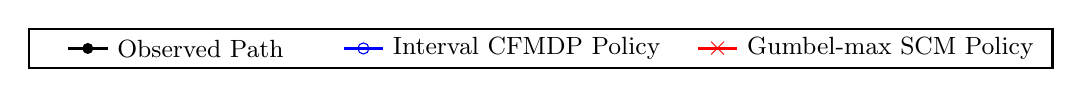
\begin{tikzpicture}[scale=1.0, every node/.style={scale=1.0}]
            \draw[thick, black] (-3, -0.25) rectangle (10, 0.25);
            %
            \draw[black, line width=1pt] (-2.5, 0.0) -- (-2,0.0);
            \fill[black] (-2.25,0.0) circle (2pt); %
            \node[right] at (-2,0.0) {\small Observed Path};
            
            %
            \draw[blue, line width=1pt] (1.0,0.0) -- (1.5,0.0);
            \node[draw=blue, circle, minimum size=4pt, inner sep=0pt] at (1.25,0.0) {}; %
            \node[right] at (1.5,0.0) {\small Interval CFMDP Policy};
            
            %
            \draw[red, line width=1pt] (5.5,0) -- (6,0);
            \node[red] at (5.75,0) {$\boldsymbol{\times}$}; %
            \node[right] at (6,0) {\small Gumbel-max SCM Policy};
        \end{tikzpicture}
    }\\
    %
    \subfigure[\footnotesize Lowest cumulative reward: Interval CFMDP ($312$), Gumbel-max SCM ($312$)]{%
        \resizebox{0.76\columnwidth}{!}{
             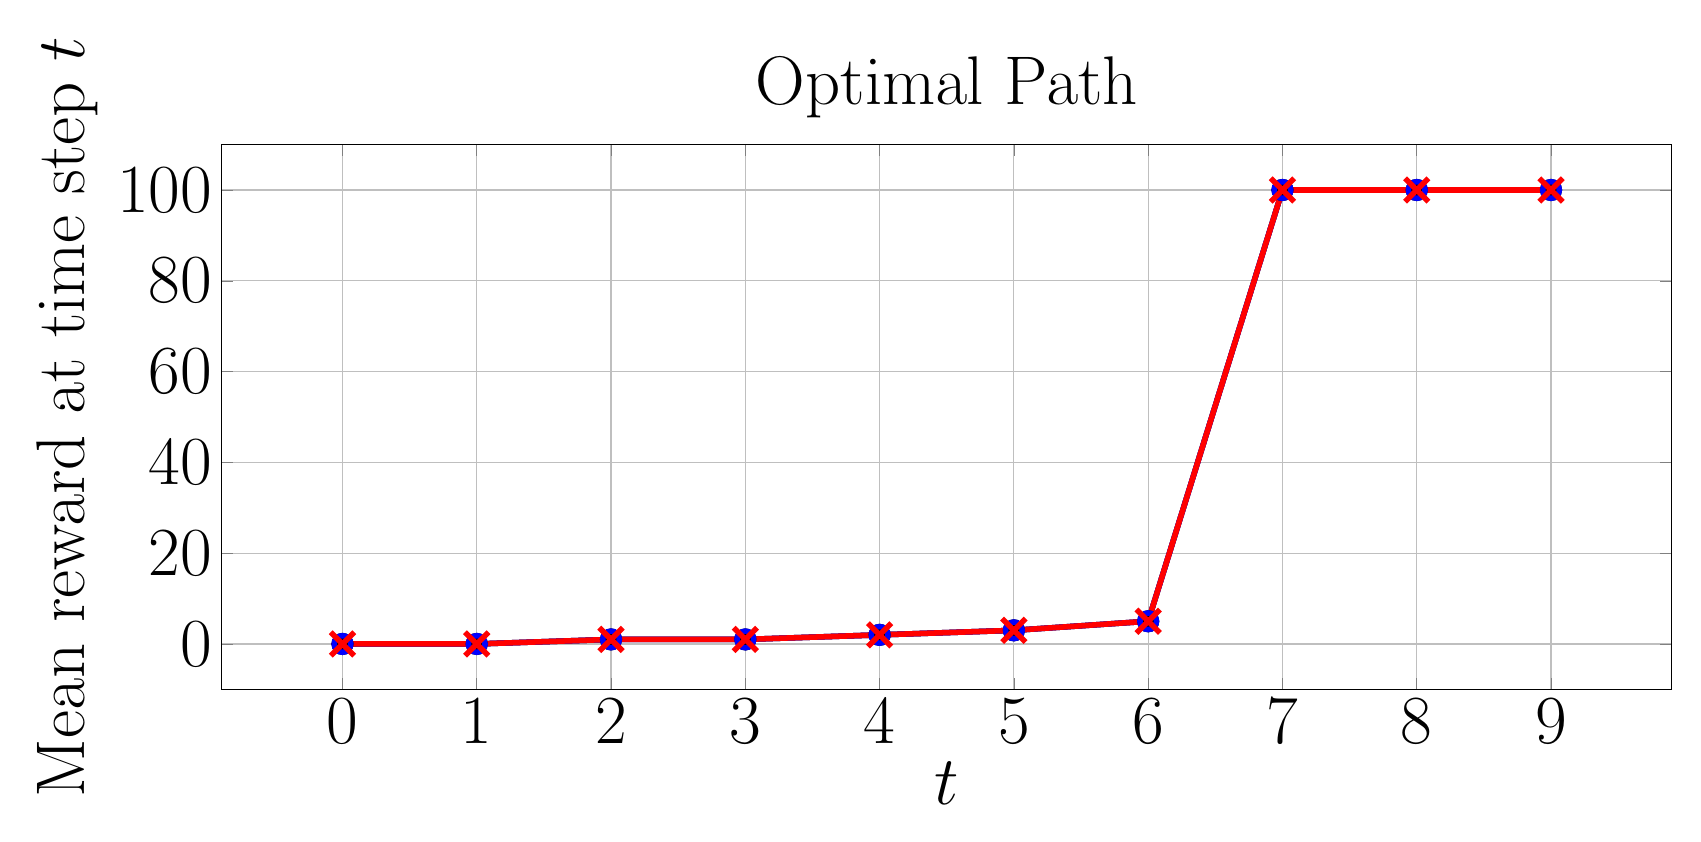
\begin{tikzpicture}
                \begin{axis}[
                    xlabel={$t$},
                    ylabel={Mean reward at time step $t$},
                    title={Optimal Path},
                    grid=both,
                    width=20cm, height=8.5cm,
                    every axis/.style={font=\Huge},
                    %
                ]
                \addplot[
                    color=black, %
                    mark=*, %
                    line width=2pt,
                    mark size=3pt,
                    error bars/.cd,
                    y dir=both, %
                    y explicit, %
                    error bar style={line width=1pt,solid},
                    error mark options={line width=1pt,mark size=4pt,rotate=90}
                ]
                coordinates {
                    (0, 0.0)  +- (0, 0.0)
                    (1, 0.0)  +- (0, 0.0) 
                    (2, 1.0)  +- (0, 0.0) 
                    (3, 1.0)  +- (0, 0.0)
                    (4, 2.0)  +- (0, 0.0)
                    (5, 3.0) +- (0, 0.0)
                    (6, 5.0) +- (0, 0.0)
                    (7, 100.0) +- (0, 0.0)
                    (8, 100.0) +- (0, 0.0)
                    (9, 100.0) +- (0, 0.0)
                };
                %
                \addplot[
                    color=blue, %
                    mark=o, %
                    line width=2pt,
                    mark size=3pt,
                    error bars/.cd,
                    y dir=both, %
                    y explicit, %
                    error bar style={line width=1pt,solid},
                    error mark options={line width=1pt,mark size=4pt,rotate=90}
                ]
                 coordinates {
                    (0, 0.0)  +- (0, 0.0)
                    (1, 0.0)  +- (0, 0.0) 
                    (2, 1.0)  +- (0, 0.0) 
                    (3, 1.0)  +- (0, 0.0)
                    (4, 2.0)  +- (0, 0.0)
                    (5, 3.0) +- (0, 0.0)
                    (6, 5.0) +- (0, 0.0)
                    (7, 100.0) +- (0, 0.0)
                    (8, 100.0) +- (0, 0.0)
                    (9, 100.0) +- (0, 0.0)
                };
                %
                \addplot[
                    color=red, %
                    mark=x, %
                    line width=2pt,
                    mark size=6pt,
                    error bars/.cd,
                    y dir=both, %
                    y explicit, %
                    error bar style={line width=1pt,solid},
                    error mark options={line width=1pt,mark size=4pt,rotate=90}
                ]
                coordinates {
                    (0, 0.0)  +- (0, 0.0)
                    (1, 0.0)  +- (0, 0.0) 
                    (2, 1.0)  +- (0, 0.0) 
                    (3, 1.0)  +- (0, 0.0)
                    (4, 2.0)  +- (0, 0.0)
                    (5, 3.0) +- (0, 0.0)
                    (6, 5.0) +- (0, 0.0)
                    (7, 100.0) +- (0, 0.0)
                    (8, 100.0) +- (0, 0.0)
                    (9, 100.0) +- (0, 0.0)
                };
                \end{axis}
            \end{tikzpicture}
         }
    }
    \hspace{1cm}
    \subfigure[\footnotesize Lowest cumulative reward: Interval CFMDP ($19$), Gumbel-max SCM ($-88$)]{%
         \resizebox{0.76\columnwidth}{!}{
            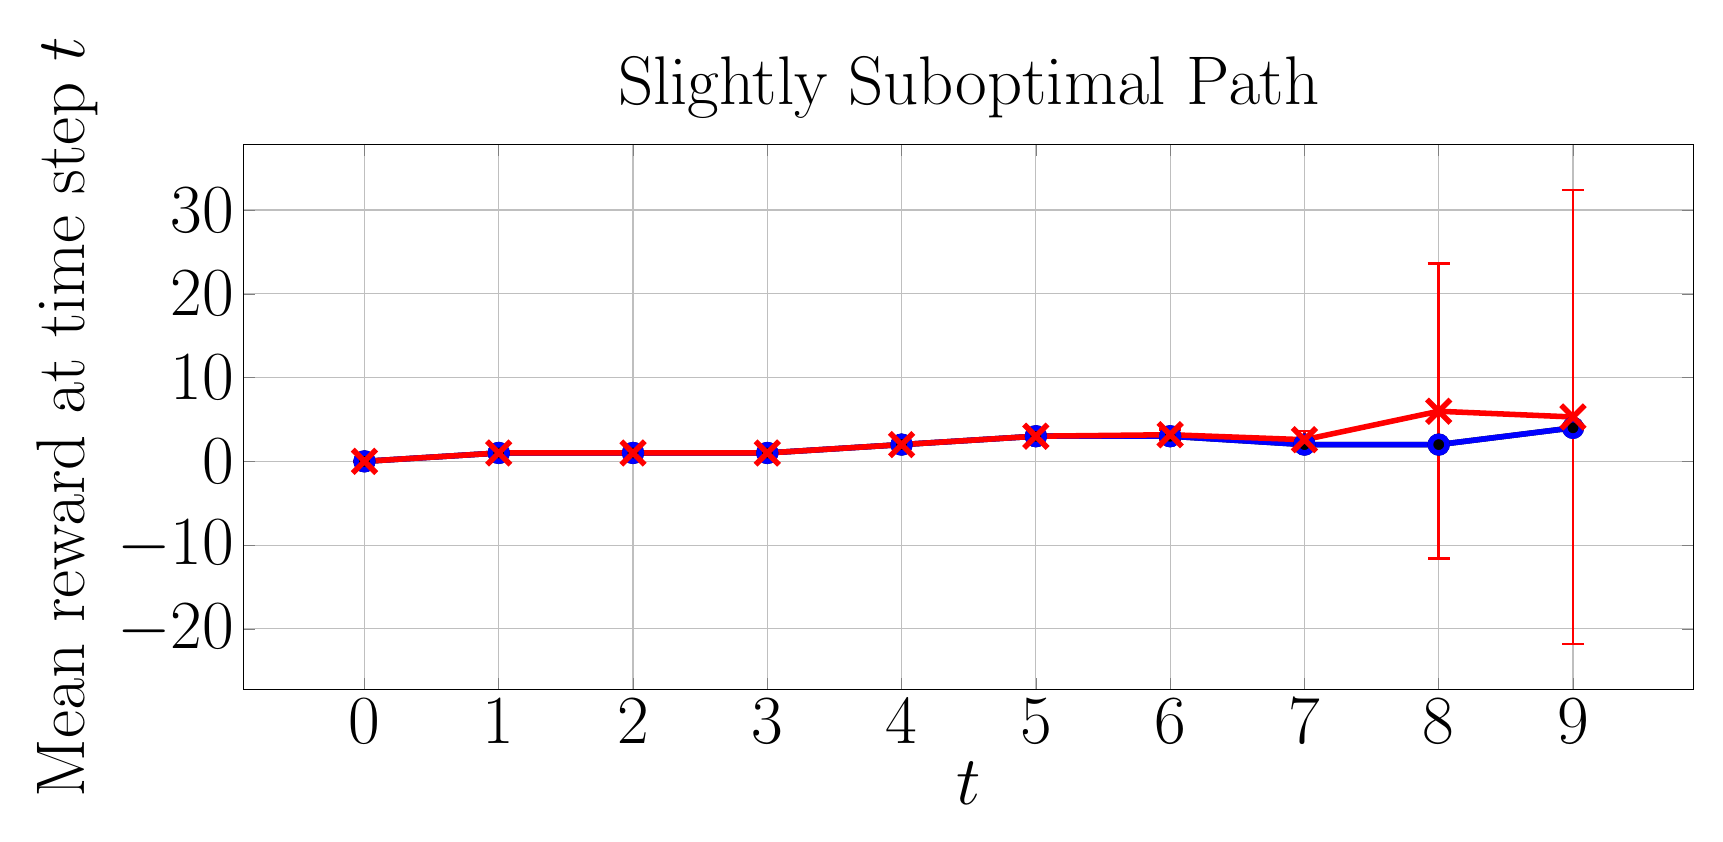
\begin{tikzpicture}
                \begin{axis}[
                    xlabel={$t$},
                    ylabel={Mean reward at time step $t$},
                    title={Slightly Suboptimal Path},
                    grid=both,
                    width=20cm, height=8.5cm,
                    every axis/.style={font=\Huge},
                    %
                ]
                \addplot[
                    color=black, %
                    mark=*, %
                    line width=2pt,
                    mark size=3pt,
                    error bars/.cd,
                    y dir=both, %
                    y explicit, %
                    error bar style={line width=1pt,solid},
                    error mark options={line width=1pt,mark size=4pt,rotate=90}
                ]
              coordinates {
                    (0, 0.0)  +- (0, 0.0)
                    (1, 1.0)  +- (0, 0.0) 
                    (2, 1.0)  +- (0, 0.0) 
                    (3, 1.0)  +- (0, 0.0)
                    (4, 2.0)  +- (0, 0.0)
                    (5, 3.0) +- (0, 0.0)
                    (6, 3.0) +- (0, 0.0)
                    (7, 2.0) +- (0, 0.0)
                    (8, 2.0) +- (0, 0.0)
                    (9, 4.0) +- (0, 0.0)
                };
                %
                \addplot[
                    color=blue, %
                    mark=o, %
                    line width=2pt,
                    mark size=3pt,
                    error bars/.cd,
                    y dir=both, %
                    y explicit, %
                    error bar style={line width=1pt,solid},
                    error mark options={line width=1pt,mark size=4pt,rotate=90}
                ]
              coordinates {
                    (0, 0.0)  +- (0, 0.0)
                    (1, 1.0)  +- (0, 0.0) 
                    (2, 1.0)  +- (0, 0.0) 
                    (3, 1.0)  +- (0, 0.0)
                    (4, 2.0)  +- (0, 0.0)
                    (5, 3.0) +- (0, 0.0)
                    (6, 3.0) +- (0, 0.0)
                    (7, 2.0) +- (0, 0.0)
                    (8, 2.0) +- (0, 0.0)
                    (9, 4.0) +- (0, 0.0)
                };
                %
                \addplot[
                    color=red, %
                    mark=x, %
                    line width=2pt,
                    mark size=6pt,
                    error bars/.cd,
                    y dir=both, %
                    y explicit, %
                    error bar style={line width=1pt,solid},
                    error mark options={line width=1pt,mark size=4pt,rotate=90}
                ]
                coordinates {
                    (0, 0.0)  +- (0, 0.0)
                    (1, 1.0)  +- (0, 0.0) 
                    (2, 1.0)  +- (0, 0.0) 
                    (3, 1.0)  +- (0, 0.0)
                    (4, 2.0)  += (0, 0.0)
                    (5, 3.0)  += (0, 0.0)
                    (6, 3.17847) += (0, 0.62606746) -= (0, 0.62606746)
                    (7, 2.5832885) += (0, 1.04598233) -= (0, 1.04598233)
                    (8, 5.978909) += (0, 17.60137623) -= (0, 17.60137623)
                    (9, 5.297059) += (0, 27.09227512) -= (0, 27.09227512)
                };
                \end{axis}
            \end{tikzpicture}
         }
    }\\[-1.5pt]
    \subfigure[\footnotesize Lowest cumulative reward: Interval CFMDP ($14$), Gumbel-max SCM ($-598$)]{%
         \resizebox{0.76\columnwidth}{!}{
             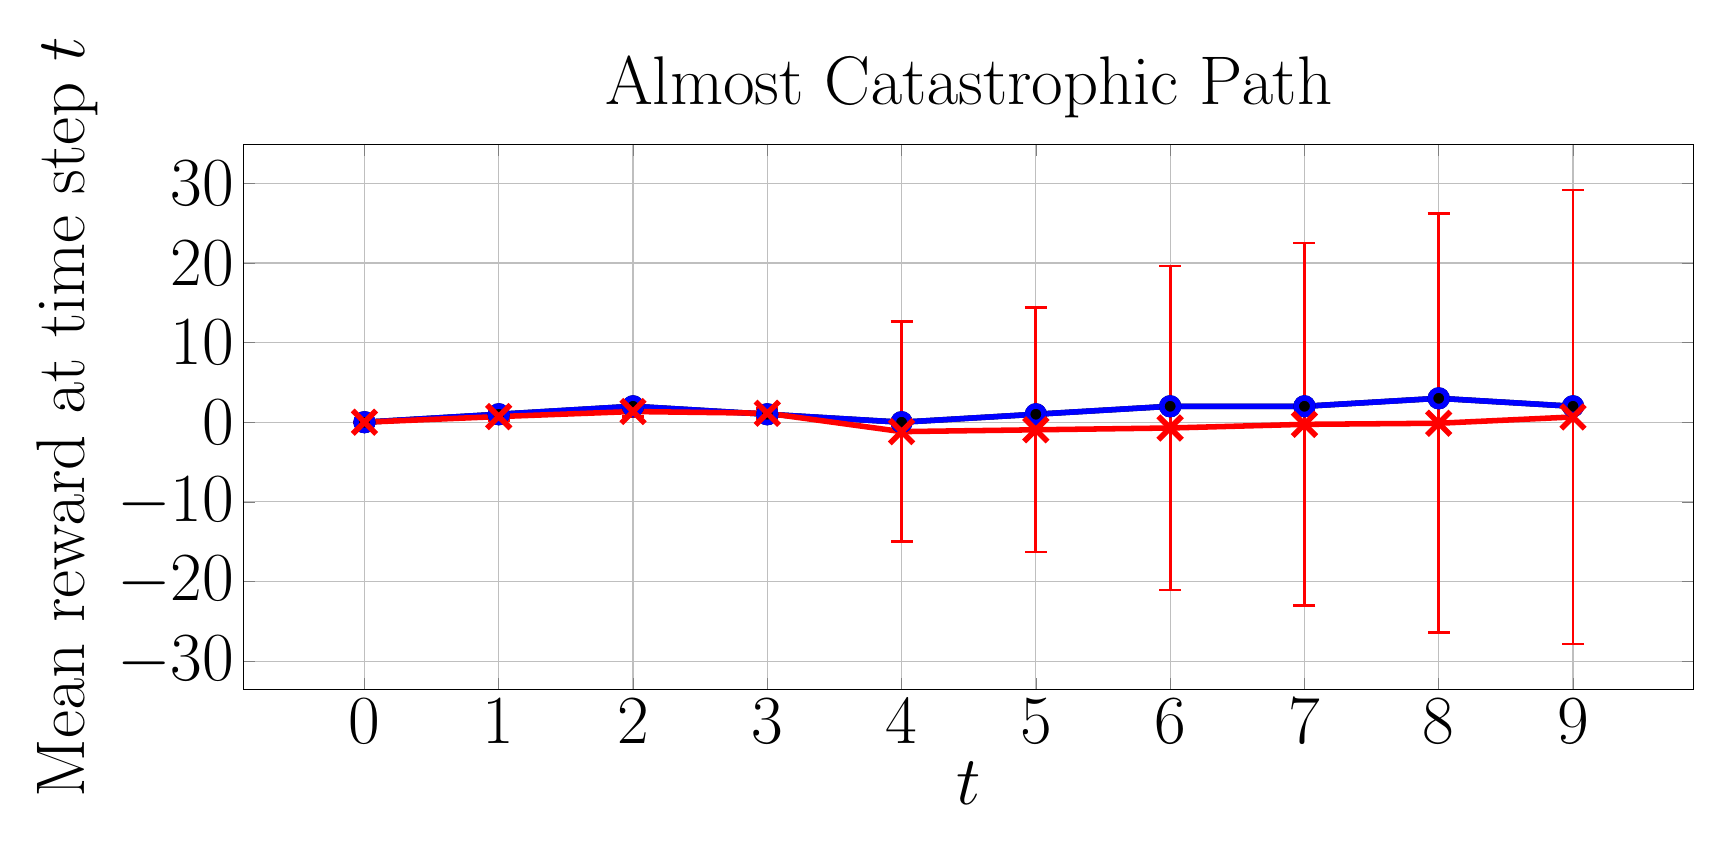
\begin{tikzpicture}
                \begin{axis}[
                    xlabel={$t$},
                    ylabel={Mean reward at time step $t$},
                    title={Almost Catastrophic Path},
                    grid=both,
                    width=20cm, height=8.5cm,
                    every axis/.style={font=\Huge},
                    %
                ]
                \addplot[
                    color=black, %
                    mark=*, %
                    line width=2pt,
                    mark size=3pt,
                    error bars/.cd,
                    y dir=both, %
                    y explicit, %
                    error bar style={line width=1pt,solid},
                    error mark options={line width=1pt,mark size=4pt,rotate=90}
                ]
                coordinates {
                    (0, 0.0)  +- (0, 0.0)
                    (1, 1.0)  +- (0, 0.0) 
                    (2, 2.0)  +- (0, 0.0) 
                    (3, 1.0)  +- (0, 0.0)
                    (4, 0.0)  +- (0, 0.0)
                    (5, 1.0) +- (0, 0.0)
                    (6, 2.0) +- (0, 0.0)
                    (7, 2.0) +- (0, 0.0)
                    (8, 3.0) +- (0, 0.0)
                    (9, 2.0) +- (0, 0.0)
                };
                %
                \addplot[
                    color=blue, %
                    mark=o, %
                    line width=2pt,
                    mark size=3pt,
                    error bars/.cd,
                    y dir=both, %
                    y explicit, %
                    error bar style={line width=1pt,solid},
                    error mark options={line width=1pt,mark size=4pt,rotate=90}
                ]
                coordinates {
                    (0, 0.0)  +- (0, 0.0)
                    (1, 1.0)  +- (0, 0.0) 
                    (2, 2.0)  +- (0, 0.0) 
                    (3, 1.0)  +- (0, 0.0)
                    (4, 0.0)  +- (0, 0.0)
                    (5, 1.0) +- (0, 0.0)
                    (6, 2.0) +- (0, 0.0)
                    (7, 2.0) +- (0, 0.0)
                    (8, 3.0) +- (0, 0.0)
                    (9, 2.0) +- (0, 0.0)
                };
                %
                \addplot[
                    color=red, %
                    mark=x, %
                    line width=2pt,
                    mark size=6pt,
                    error bars/.cd,
                    y dir=both, %
                    y explicit, %
                    error bar style={line width=1pt,solid},
                    error mark options={line width=1pt,mark size=4pt,rotate=90}
                ]
                coordinates {
                    (0, 0.0)  +- (0, 0.0)
                    (1, 0.7065655)  +- (0, 0.4553358) 
                    (2, 1.341673)  +- (0, 0.67091621) 
                    (3, 1.122926)  +- (0, 0.61281824)
                    (4, -1.1821935)  +- (0, 13.82444042)
                    (5, -0.952399)  +- (0, 15.35195457)
                    (6, -0.72672) +- (0, 20.33508414)
                    (7, -0.268983) +- (0, 22.77861454)
                    (8, -0.1310835) +- (0, 26.31013314)
                    (9, 0.65806) +- (0, 28.50670214)
                };
                %
            %
            %
            %
            %
            %
            %
            %
            %
            %
            %
            %
            %
            %
            %
            %
            %
            %
            %
                \end{axis}
            \end{tikzpicture}
         }
    }
    \hspace{1cm}
    \subfigure[\footnotesize Lowest cumulative reward: Interval CFMDP ($-698$), Gumbel-max SCM ($-698$)]{%
         \resizebox{0.76\columnwidth}{!}{
            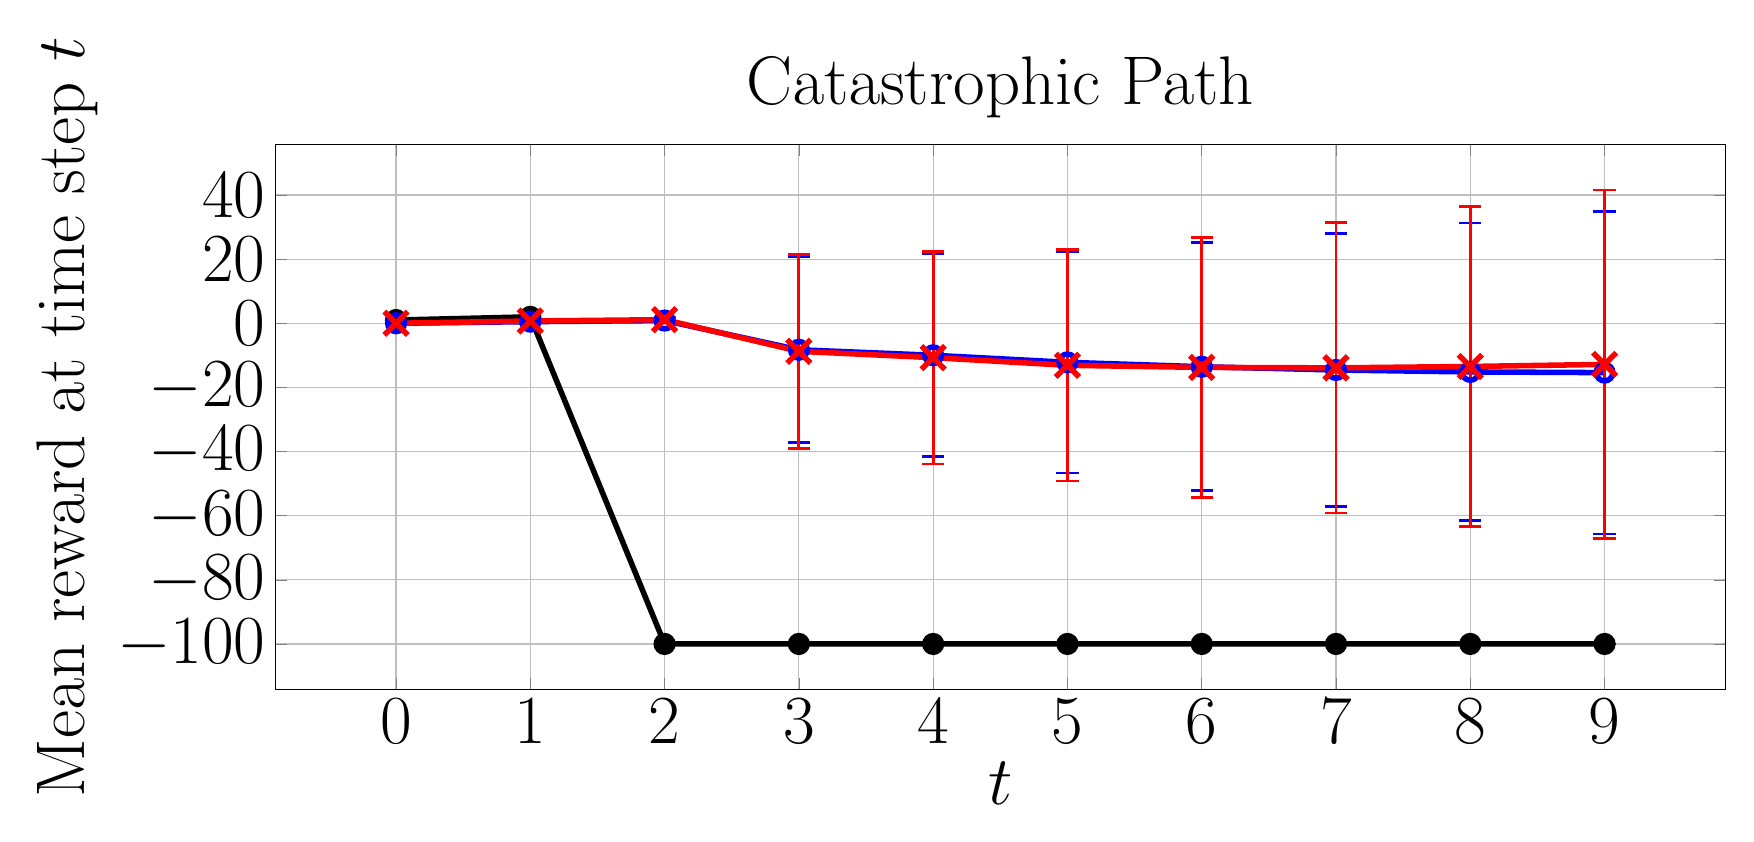
\begin{tikzpicture}
                \begin{axis}[
                    xlabel={$t$},
                    ylabel={Mean reward at time step $t$},
                    title={Catastrophic Path},
                    grid=both,
                    width=20cm, height=8.5cm,
                    every axis/.style={font=\Huge},
                    %
                ]
                \addplot[
                    color=black, %
                    mark=*, %
                    line width=2pt,
                    mark size=3pt,
                    error bars/.cd,
                    y dir=both, %
                    y explicit, %
                    error bar style={line width=1pt,solid},
                    error mark options={line width=1pt,mark size=4pt,rotate=90}
                ]
                coordinates {
                    (0, 1.0)  +- (0, 0.0)
                    (1, 2.0)  +- (0, 0.0) 
                    (2, -100.0)  +- (0, 0.0) 
                    (3, -100.0)  +- (0, 0.0)
                    (4, -100.0)  +- (0, 0.0)
                    (5, -100.0) +- (0, 0.0)
                    (6, -100.0) +- (0, 0.0)
                    (7, -100.0) +- (0, 0.0)
                    (8, -100.0) +- (0, 0.0)
                    (9, -100.0) +- (0, 0.0)
                };
                %
                \addplot[
                    color=blue, %
                    mark=o, %
                    line width=2pt,
                    mark size=3pt,
                    error bars/.cd,
                    y dir=both, %
                    y explicit, %
                    error bar style={line width=1pt,solid},
                    error mark options={line width=1pt,mark size=4pt,rotate=90}
                ]
                coordinates {
                    (0, 0.0)  +- (0, 0.0)
                    (1, 0.504814)  +- (0, 0.49997682) 
                    (2, 0.8439835)  +- (0, 0.76831917) 
                    (3, -8.2709165)  +- (0, 28.93656754)
                    (4, -9.981082)  +- (0, 31.66825363)
                    (5, -12.1776325) +- (0, 34.53463233)
                    (6, -13.556076) +- (0, 38.62845372)
                    (7, -14.574418) +- (0, 42.49603359)
                    (8, -15.1757075) +- (0, 46.41913968)
                    (9, -15.3900395) +- (0, 50.33563368)
                };
                %
                \addplot[
                    color=red, %
                    mark=x, %
                    line width=2pt,
                    mark size=6pt,
                    error bars/.cd,
                    y dir=both, %
                    y explicit, %
                    error bar style={line width=1pt,solid},
                    error mark options={line width=1pt,mark size=4pt,rotate=90}
                ]
                coordinates {
                    (0, 0.0)  +- (0, 0.0)
                    (1, 0.701873)  +- (0, 0.45743556) 
                    (2, 1.1227805)  +- (0, 0.73433129) 
                    (3, -8.7503255)  +- (0, 30.30257976)
                    (4, -10.722092)  +- (0, 33.17618589)
                    (5, -13.10721)  +- (0, 36.0648089)
                    (6, -13.7631645) +- (0, 40.56553451)
                    (7, -13.909043) +- (0, 45.23829402)
                    (8, -13.472517) +- (0, 49.96270296)
                    (9, -12.8278835) +- (0, 54.38618735)
                };
                %
            %
            %
            %
            %
            %
            %
            %
            %
            %
            %
            %
            %
            %
            %
            %
            %
            %
            %
                \end{axis}
            \end{tikzpicture}
         }
    }
    \caption{Average instant reward of CF paths induced by policies on GridWorld $p=0.4$.}
    \label{fig: reward p=0.4}
\end{figure*}

\subsection{Experimental Setup}
To compare policy performance, we measure the average rewards of counterfactual paths induced by our policy and the Gumbel-max policy by uniformly sampling $200$ counterfactual MDPs from the ICFMDP and generating $10,000$ counterfactual paths over each sampled CFMDP. \jl{Since the interval CFMDP depends on the observed path, we select $4$  paths of varying optimality to evaluate how the observed path impacts the performance of both policies: an optimal path, a slightly suboptimal path that could reach the optimal reward with a few changes, a catastrophic path that enters a catastrophic, terminal state with low reward, and an almost catastrophic path that was close to entering a catastrophic state.} When measuring the average probability bound widths and execution time needed to generate the ICFMDPs, we averaged over $20$ randomly generated observed paths
\footnote{Further training details are provided in Appendix \ref{app: training details}, and the code is provided at \href{https://github.com/ddv-lab/robust-cf-inference-in-MDPs}{https://github.com/ddv-lab/robust-cf-inference-in-MDPs}
%
%
.}.

\subsection{GridWorld}
\jl{The GridWorld MDP is a $4 \times 4$ grid where an agent must navigate from the top-left corner to the goal state in the bottom-right corner, avoiding a dangerous terminal state in the centre. At each time step, the agent can move up, down, left, or right, but there is a small probability (controlled by hyper-parameter $p$) of moving in an unintended direction. As the agent nears the goal, the reward for each state increases, culminating in a reward of $+100$ for reaching the goal. Entering the dangerous state results in a penalty of $-100$. We use two versions of GridWorld: a less stochastic version with $p=0.9$ (i.e., $90$\% chance of moving in the chosen direction) and a more stochastic version with $p=0.4$.}

\paragraph{GridWorld ($p=0.9$)}
When $p=0.9$, the counterfactual probability bounds are typically narrow (see Table \ref{tab:nonzero_probs} for average measurements). Consequently, as shown in Figure \ref{fig: reward p=0.9}, both policies are nearly identical and perform similarly well across the optimal, slightly suboptimal, and catastrophic paths.
%
However, for the almost catastrophic path, the interval CFMDP path is more conservative and follows the observed path more closely (as this is where the probability bounds are narrowest), which typically requires one additional step to reach the goal state than the Gumbel-max SCM policy.
%

\paragraph{GridWorld ($p=0.4$)}
\jl{When $p=0.4$, the GridWorld environment becomes more uncertain, increasing the risk of entering the dangerous state even if correct actions are chosen. Thus, as shown in Figure \ref{fig: reward p=0.4}, the interval CFMDP policy adopts a more conservative approach, avoiding deviation from the observed policy if it cannot guarantee higher counterfactual rewards (see the slightly suboptimal and almost catastrophic paths), whereas the Gumbel-max SCM is inconsistent: it can yield higher rewards, but also much lower rewards, reflected in the wide error bars.} For the catastrophic path, both policies must deviate from the observed path to achieve a higher reward and, in this case, perform similarly.
%
%
%
%
\subsection{Sepsis}
The Sepsis MDP \citep{oberst2019counterfactual} simulates trajectories of Sepsis patients. Each state consists of four vital signs (heart rate, blood pressure, oxygen concentration, and glucose levels), categorised as low, normal, or high.
and three treatments that can be toggled on/off at each time step (8 actions in total). Unlike \citet{oberst2019counterfactual}, we scale rewards based on the number of out-of-range vital signs, between $-1000$ (patient dies) and $1000$ (patient discharged). \jl{Like the GridWorld $p=0.4$ experiment, the Sepsis MDP is highly uncertain, as many states are equally likely to lead to optimal and poor outcomes. Thus, as shown in Figure \ref{fig: reward sepsis}, both policies follow the observed optimal and almost catastrophic paths to guarantee rewards are no worse than the observation.} However, improving the catastrophic path requires deviating from the observation. Here, the Gumbel-max SCM policy, on average, performs better than the interval CFMDP policy. But, since both policies have lower bounds clipped at $-1000$, neither policy reliably improves over the observation. In contrast, for the slightly suboptimal path, the interval CFMDP policy performs significantly better, shown by its higher lower bounds. 
Moreover, in these two cases, the worst-case counterfactual path generated by the interval CFMDP policy is better than that of the Gumbel-max SCM policy,
indicating its greater robustness.
%
\begin{figure*}
    \centering
     \resizebox{0.6\textwidth}{!}{
        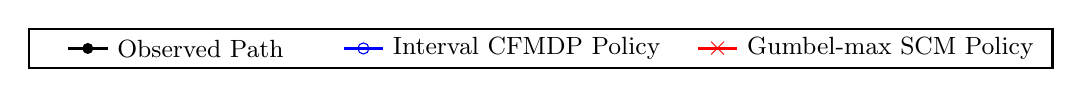
\begin{tikzpicture}[scale=1.0, every node/.style={scale=1.0}]
            \draw[thick, black] (-3, -0.25) rectangle (10, 0.25);
            %
            \draw[black, line width=1pt] (-2.5, 0.0) -- (-2,0.0);
            \fill[black] (-2.25,0.0) circle (2pt); %
            \node[right] at (-2,0.0) {\small Observed Path};
            
            %
            \draw[blue, line width=1pt] (1.0,0.0) -- (1.5,0.0);
            \node[draw=blue, circle, minimum size=4pt, inner sep=0pt] at (1.25,0.0) {}; %
            \node[right] at (1.5,0.0) {\small Interval CFMDP Policy};
            
            %
            \draw[red, line width=1pt] (5.5,0) -- (6,0);
            \node[red] at (5.75,0) {$\boldsymbol{\times}$}; %
            \node[right] at (6,0) {\small Gumbel-max SCM Policy};
        \end{tikzpicture}
    }\\
    \subfigure[\footnotesize Lowest cumulative reward: Interval CFMDP ($8000$), Gumbel-max SCM ($8000$)]{%
         \resizebox{0.76\columnwidth}{!}{
             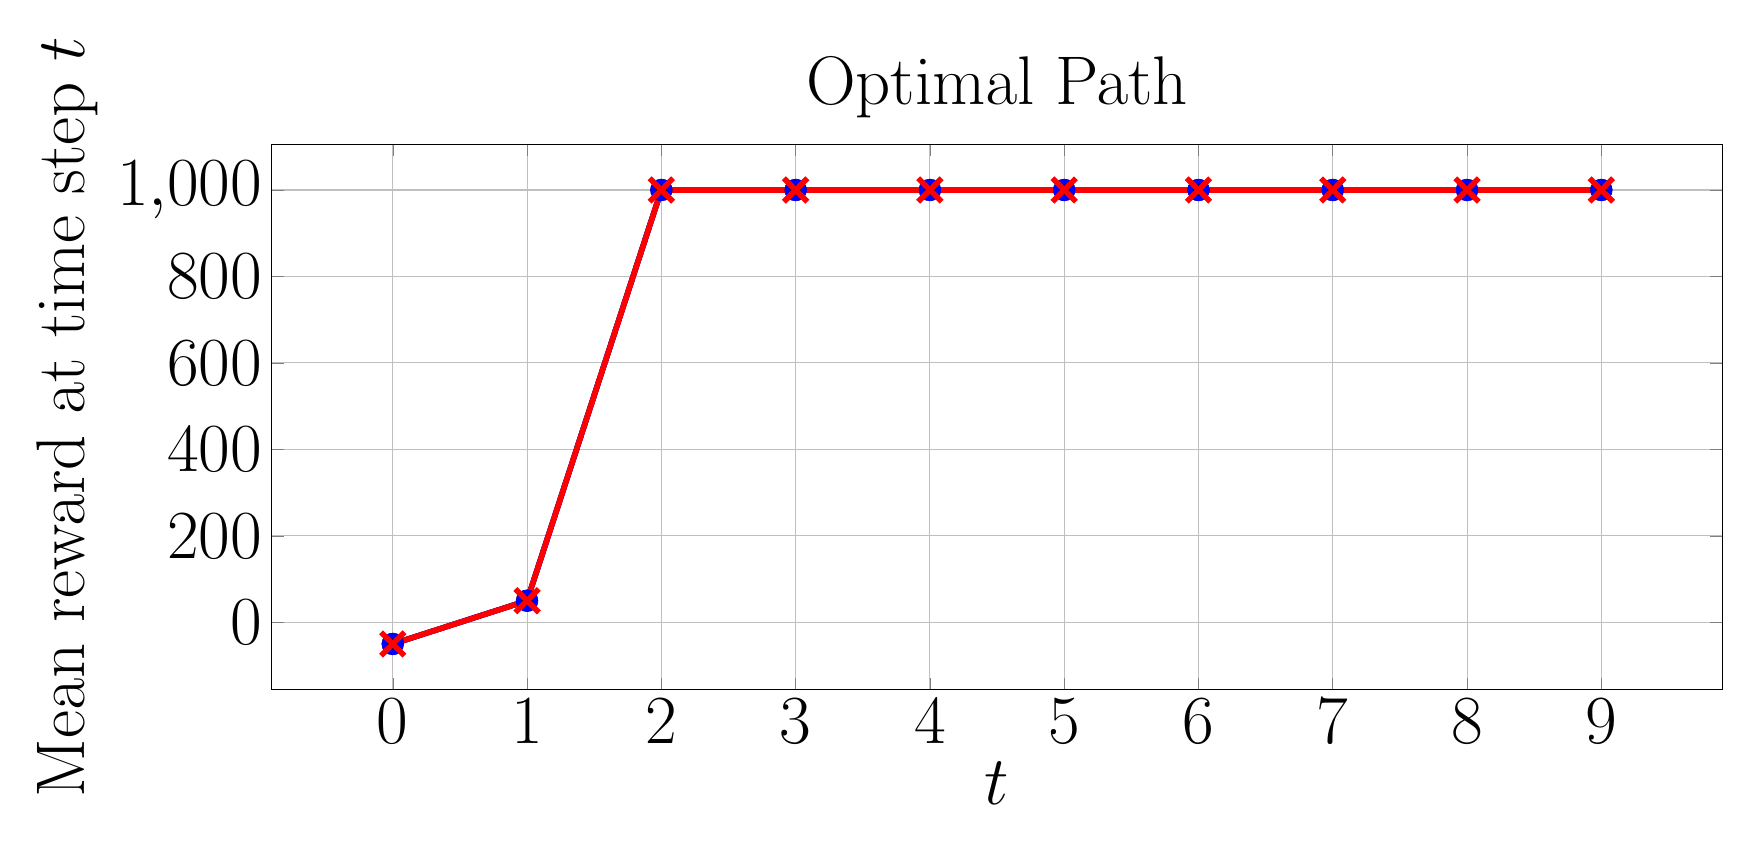
\begin{tikzpicture}
                \begin{axis}[
                    xlabel={$t$},
                    ylabel={Mean reward at time step $t$},
                    title={Optimal Path},
                    grid=both,
                    width=20cm, height=8.5cm,
                    every axis/.style={font=\Huge},
                    %
                ]
                \addplot[
                    color=black, %
                    mark=*, %
                    line width=2pt,
                    mark size=3pt,
                ]
                coordinates {
                    (0, -50.0)
                    (1, 50.0)
                    (2, 1000.0)
                    (3, 1000.0)
                    (4, 1000.0)
                    (5, 1000.0)
                    (6, 1000.0)
                    (7, 1000.0)
                    (8, 1000.0)
                    (9, 1000.0)
                };
                %
                \addplot[
                    color=blue, %
                    mark=o, %
                    line width=2pt,
                    mark size=3pt,
                    error bars/.cd,
                    y dir=both, %
                    y explicit, %
                    error bar style={line width=1pt,solid},
                    error mark options={line width=1pt,mark size=4pt,rotate=90}
                ]
                coordinates {
                    (0, -50.0)  +- (0, 0.0)
                    (1, 50.0)  +- (0, 0.0) 
                    (2, 1000.0)  +- (0, 0.0) 
                    (3, 1000.0)  +- (0, 0.0)
                    (4, 1000.0)  +- (0, 0.0)
                    (5, 1000.0) +- (0, 0.0)
                    (6, 1000.0) +- (0, 0.0)
                    (7, 1000.0) +- (0, 0.0)
                    (8, 1000.0) +- (0, 0.0)
                    (9, 1000.0) +- (0, 0.0)
                };
                %
                \addplot[
                    color=red, %
                    mark=x, %
                    line width=2pt,
                    mark size=6pt,
                    error bars/.cd,
                    y dir=both, %
                    y explicit, %
                    error bar style={line width=1pt,solid},
                    error mark options={line width=1pt,mark size=4pt,rotate=90}
                ]
                coordinates {
                    (0, -50.0)  +- (0, 0.0)
                    (1, 50.0)  +- (0, 0.0) 
                    (2, 1000.0)  +- (0, 0.0) 
                    (3, 1000.0)  +- (0, 0.0)
                    (4, 1000.0)  +- (0, 0.0)
                    (5, 1000.0) +- (0, 0.0)
                    (6, 1000.0) +- (0, 0.0)
                    (7, 1000.0) +- (0, 0.0)
                    (8, 1000.0) +- (0, 0.0)
                    (9, 1000.0) +- (0, 0.0)
                };
                %
                \end{axis}
            \end{tikzpicture}
         }
    }
    \hspace{1cm}
    \subfigure[\footnotesize Lowest cumulative reward: Interval CFMDP ($-5980$), Gumbel-max SCM ($-8000$)]{%
         \resizebox{0.76\columnwidth}{!}{
            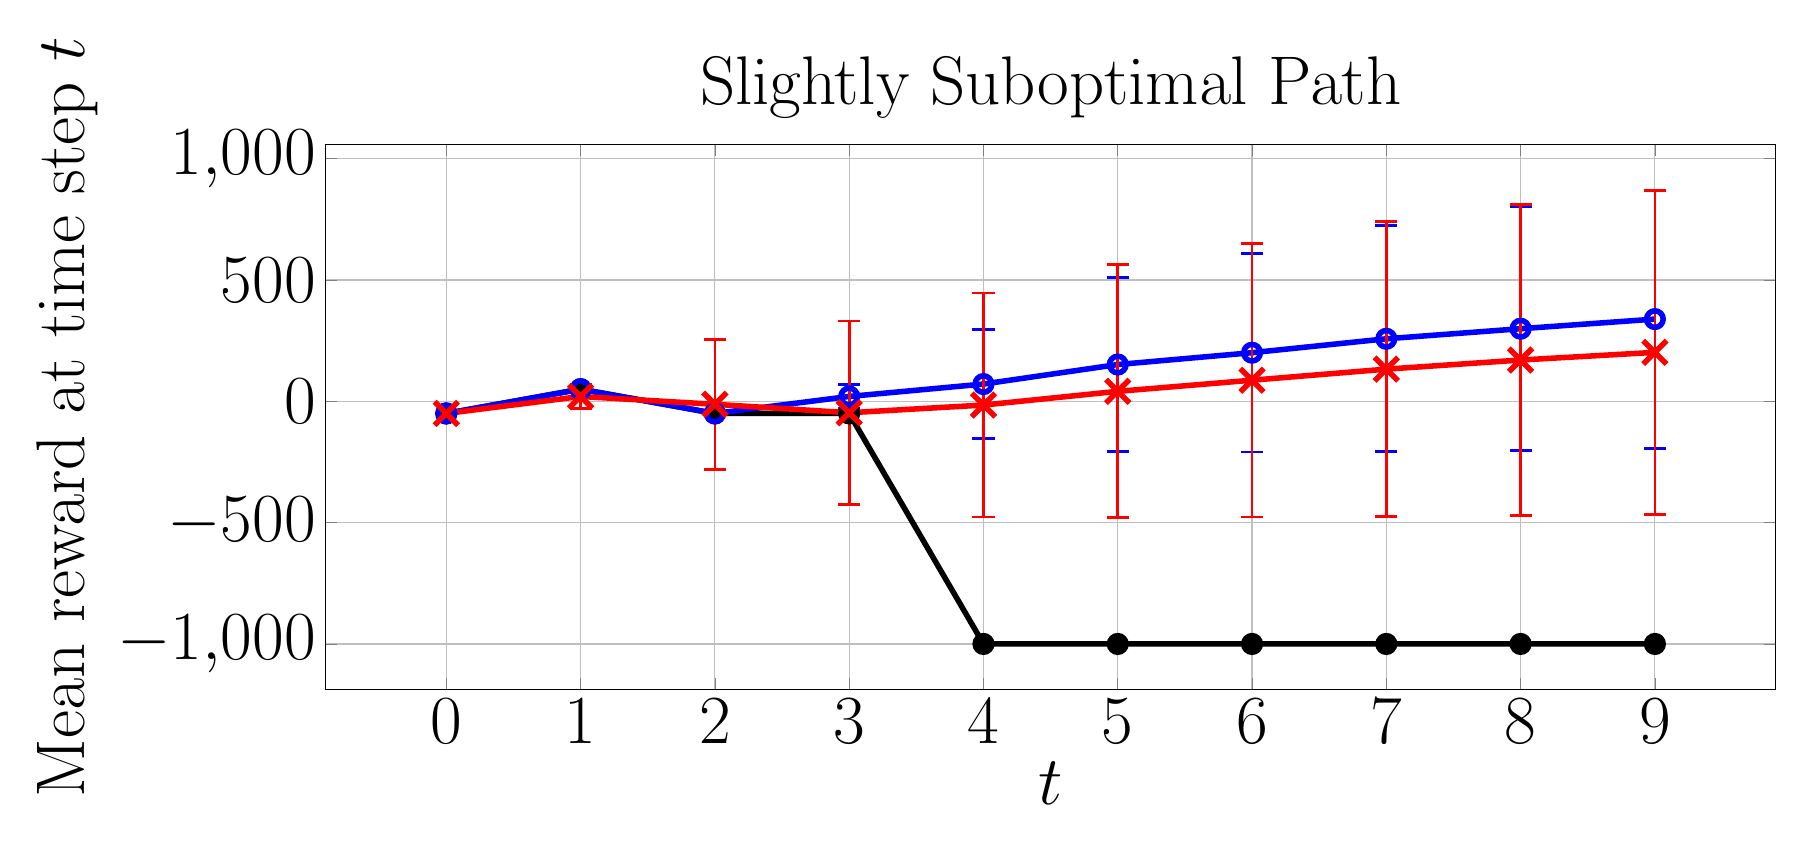
\begin{tikzpicture}
                \begin{axis}[
                    xlabel={$t$},
                    ylabel={Mean reward at time step $t$},
                    title={Slightly Suboptimal Path},
                    grid=both,
                    width=20cm, height=8.5cm,
                    every axis/.style={font=\Huge},
                    %
                ]
               \addplot[
                    color=black, %
                    mark=*, %
                    line width=2pt,
                    mark size=3pt,
                ]
                coordinates {
                    (0, -50.0)
                    (1, 50.0)
                    (2, -50.0)
                    (3, -50.0)
                    (4, -1000.0)
                    (5, -1000.0)
                    (6, -1000.0)
                    (7, -1000.0)
                    (8, -1000.0)
                    (9, -1000.0)
                };
                %
                \addplot[
                    color=blue, %
                    mark=o, %
                    line width=2pt,
                    mark size=3pt,
                    error bars/.cd,
                    y dir=both, %
                    y explicit, %
                    error bar style={line width=1pt,solid},
                    error mark options={line width=1pt,mark size=4pt,rotate=90}
                ]
                coordinates {
                    (0, -50.0)  +- (0, 0.0)
                    (1, 50.0)  +- (0, 0.0) 
                    (2, -50.0)  +- (0, 0.0) 
                    (3, 20.0631)  +- (0, 49.97539413)
                    (4, 71.206585)  +- (0, 226.02033693)
                    (5, 151.60797) +- (0, 359.23292559)
                    (6, 200.40593) +- (0, 408.86185176)
                    (7, 257.77948) +- (0, 466.10372804)
                    (8, 299.237465) +- (0, 501.82579506)
                    (9, 338.9129) +- (0, 532.06124996)
                };
                %
                \addplot[
                    color=red, %
                    mark=x, %
                    line width=2pt,
                    mark size=6pt,
                    error bars/.cd,
                    y dir=both, %
                    y explicit, %
                    error bar style={line width=1pt,solid},
                    error mark options={line width=1pt,mark size=4pt,rotate=90}
                ]
                coordinates {
                    (0, -50.0)  +- (0, 0.0)
                    (1, 20.00736)  +- (0, 49.99786741) 
                    (2, -12.282865)  +- (0, 267.598755) 
                    (3, -47.125995)  +- (0, 378.41755832)
                    (4, -15.381965)  +- (0, 461.77616558)
                    (5, 41.15459) +- (0, 521.53189262)
                    (6, 87.01595) +- (0, 564.22243126 )
                    (7, 132.62376) +- (0, 607.31338037)
                    (8, 170.168145) +- (0, 641.48013693)
                    (9, 201.813135) +- (0, 667.29441777)
                };
                %
                %
                %
                %
                %
                %
                %
                %
                %
                %
                %
                %
                %
                %
                %
                %
                %
                %
                %
                \end{axis}
            \end{tikzpicture}
         }
    }\\[-1.5pt]
    \subfigure[\footnotesize Lowest cumulative reward: Interval CFMDP ($100$), Gumbel-max SCM ($100$)]{%
         \resizebox{0.76\columnwidth}{!}{
             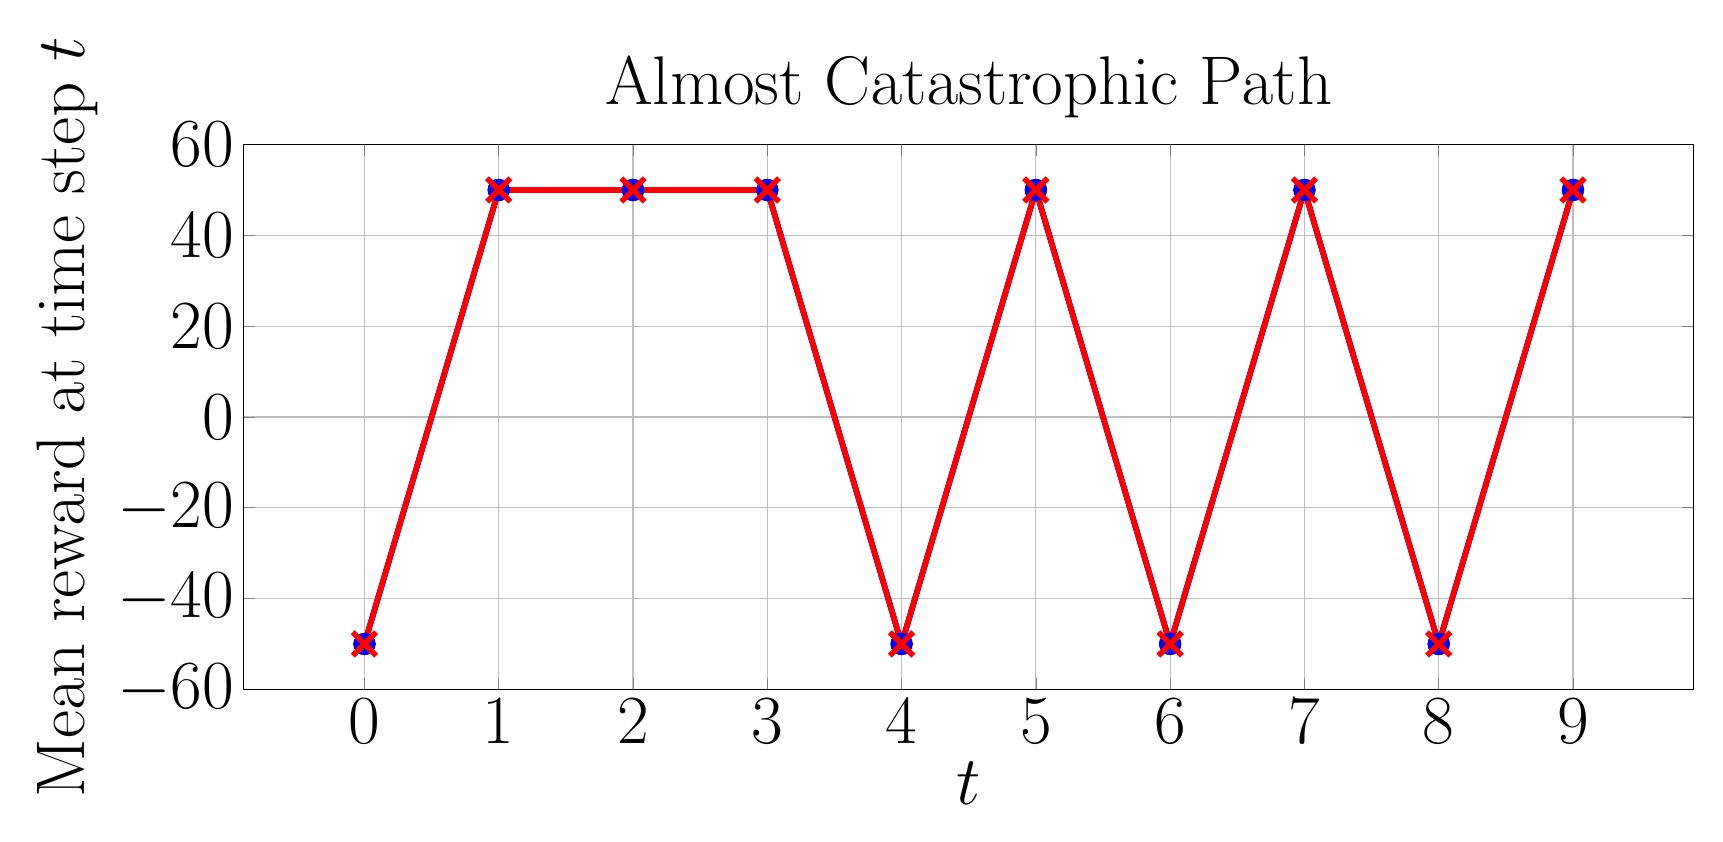
\begin{tikzpicture}
                \begin{axis}[
                    xlabel={$t$},
                    ylabel={Mean reward at time step $t$},
                    title={Almost Catastrophic Path},
                    grid=both,
                    every axis/.style={font=\Huge},
                    width=20cm, height=8.5cm,
                    %
                ]
               \addplot[
                    color=black, %
                    mark=*, %
                    line width=2pt,
                    mark size=3pt,
                ]
                coordinates {
                    (0, -50.0)
                    (1, 50.0)
                    (2, 50.0)
                    (3, 50.0)
                    (4, -50.0)
                    (5, 50.0)
                    (6, -50.0)
                    (7, 50.0)
                    (8, -50.0)
                    (9, 50.0)
                };
                %
                %
                \addplot[
                    color=blue, %
                    mark=o, %
                    line width=2pt,
                    mark size=3pt,
                    error bars/.cd,
                    y dir=both, %
                    y explicit, %
                    error bar style={line width=1pt,solid},
                    error mark options={line width=1pt,mark size=4pt,rotate=90}
                ]
                coordinates {
                    (0, -50.0)  +- (0, 0.0)
                    (1, 50.0)  +- (0, 0.0) 
                    (2, 50.0)  +- (0, 0.0) 
                    (3, 50.0)  +- (0, 0.0)
                    (4, -50.0)  +- (0, 0.0)
                    (5, 50.0) +- (0, 0.0)
                    (6, -50.0) +- (0, 0.0)
                    (7, 50.0) +- (0, 0.0)
                    (8, -50.0) +- (0, 0.0)
                    (9, 50.0) +- (0, 0.0)
                };
                %
                \addplot[
                    color=red, %
                    mark=x, %
                    line width=2pt,
                    mark size=6pt,
                    error bars/.cd,
                    y dir=both, %
                    y explicit, %
                    error bar style={line width=1pt,solid},
                    error mark options={line width=1pt,mark size=4pt,rotate=90}
                ]
                coordinates {
                    (0, -50.0)  +- (0, 0.0)
                    (1, 50.0)  +- (0, 0.0) 
                    (2, 50.0)  +- (0, 0.0) 
                    (3, 50.0)  +- (0, 0.0)
                    (4, -50.0)  +- (0, 0.0)
                    (5, 50.0) +- (0, 0.0)
                    (6, -50.0) +- (0, 0.0)
                    (7, 50.0) +- (0, 0.0)
                    (8, -50.0) +- (0, 0.0)
                    (9, 50.0) +- (0, 0.0)
                };
                %
                %
                %
                %
                %
                %
                %
                %
                %
                %
                %
                %
                %
                %
                %
                %
                %
                %
                %
                \end{axis}
            \end{tikzpicture}
         }
    }
    \hspace{1cm}
    \subfigure[\footnotesize Lowest cumulative reward: Interval CFMDP ($-7150$), Gumbel-max SCM ($-9050$)]{%
         \resizebox{0.76\columnwidth}{!}{
            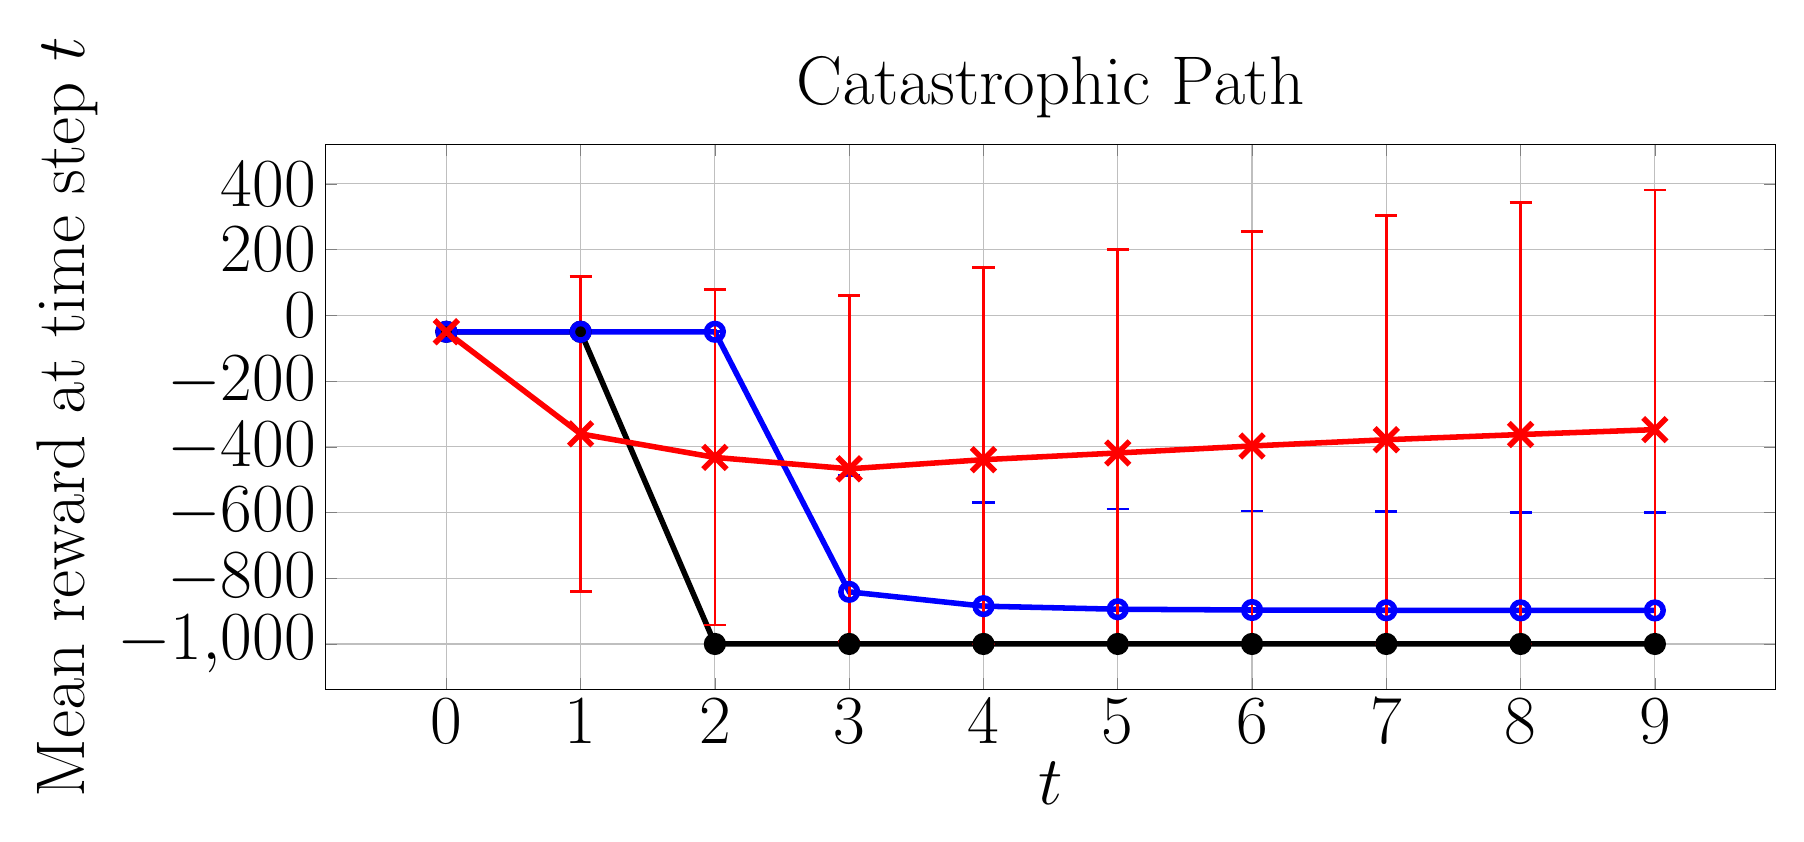
\begin{tikzpicture}
                \begin{axis}[
                    xlabel={$t$},
                    ylabel={Mean reward at time step $t$},
                    title={Catastrophic Path},
                    grid=both,
                    width=20cm, height=8.5cm,
                    every axis/.style={font=\Huge},
                    %
                ]
               \addplot[
                    color=black, %
                    mark=*, %
                    line width=2pt,
                    mark size=3pt,
                ]
                coordinates {
                    (0, -50.0)
                    (1, -50.0)
                    (2, -1000.0)
                    (3, -1000.0)
                    (4, -1000.0)
                    (5, -1000.0)
                    (6, -1000.0)
                    (7, -1000.0)
                    (8, -1000.0)
                    (9, -1000.0)
                };
                %
                %
                \addplot[
                    color=blue, %
                    mark=o, %
                    line width=2pt,
                    mark size=3pt,
                    error bars/.cd,
                    y dir=both, %
                    y explicit, %
                    error bar style={line width=1pt,solid},
                    error mark options={line width=1pt,mark size=4pt,rotate=90}
                ]
                coordinates {
                    (0, -50.0)  +- (0, 0.0)
                    (1, -50.0)  +- (0, 0.0) 
                    (2, -50.0)  +- (0, 0.0) 
                    (3, -841.440725)  += (0, 354.24605512) -= (0, 158.559275)
                    (4, -884.98225)  += (0, 315.37519669) -= (0, 115.01775)
                    (5, -894.330425) += (0, 304.88572805) -= (0, 105.669575)
                    (6, -896.696175) += (0, 301.19954514) -= (0, 103.303825)
                    (7, -897.4635) += (0, 299.61791279) -= (0, 102.5365)
                    (8, -897.77595) += (0, 298.80392585) -= (0, 102.22405)
                    (9, -897.942975) += (0, 298.32920557) -= (0, 102.057025)
                };
                %
                \addplot[
                    color=red, %
                    mark=x, %
                    line width=2pt,
                    mark size=6pt,
                    error bars/.cd,
                    y dir=both, %
                    y explicit, %
                    error bar style={line width=1pt,solid},
                    error mark options={line width=1pt,mark size=4pt,rotate=90}
                ]
            coordinates {
                    (0, -50.0)  +- (0, 0.0)
                    (1, -360.675265)  +- (0, 479.39812699) 
                    (2, -432.27629)  +- (0, 510.38620897) 
                    (3, -467.029545)  += (0, 526.36009628) -= (0, 526.36009628)
                    (4, -439.17429)  += (0, 583.96638919) -= (0, 560.82571)
                    (5, -418.82704) += (0, 618.43027478) -= (0, 581.17296)
                    (6, -397.464895) += (0, 652.67322574) -= (0, 602.535105)
                    (7, -378.49052) += (0, 682.85407033) -= (0, 621.50948)
                    (8, -362.654195) += (0, 707.01412023) -= (0, 637.345805)
                    (9, -347.737935) += (0, 729.29076479) -= (0, 652.262065)
                };
                %
                %
                %
                %
                %
                %
                %
                %
                %
                %
                %
                %
                %
                %
                %
                %
                %
                %
                %
                \end{axis}
            \end{tikzpicture}
         }
    }
    \caption{Average instant reward of CF paths induced by policies on Sepsis.}
    \label{fig: reward sepsis}
\end{figure*}

%
%
%
\subsection{Interval CFMDP Bounds}
%
%
Table \ref{tab:nonzero_probs} presents the mean counterfactual probability bound widths (excluding transitions where the upper bound is $0$) for each MDP, averaged over 20 observed paths. We compare the bounds under counterfactual stability (CS) and monotonicity (M) assumptions, CS alone, and no assumptions. This shows that the assumptions marginally reduce the bound widths, indicating the assumptions tighten the bounds without excluding too many causal models, as intended.
\renewcommand{\arraystretch}{1}

\begin{table}
\centering
\caption{Mean width of counterfactual probability bounds}
\resizebox{0.8\columnwidth}{!}{%
\begin{tabular}{|c|c|c|c|}
\hline
\multirow{2}{*}{\textbf{Environment}} & \multicolumn{3}{c|}{\textbf{Assumptions}} \\ \cline{2-4}
 & \textbf{CS + M} & \textbf{CS} & \textbf{None\tablefootnote{\jl{Equivalent to \citet{li2024probabilities}'s bounds (see Section \ref{sec: equivalence with Li}).}}} \\ \hline
\textbf{GridWorld} ($p=0.9$) & 0.0817 & 0.0977 & 0.100 \\ \hline
\textbf{GridWorld} ($p=0.4$) & 0.552  & 0.638  & 0.646 \\ \hline
\textbf{Sepsis} & 0.138 & 0.140 & 0.140 \\ \hline
\end{tabular}
}
\label{tab:nonzero_probs}
\end{table}


\subsection{Execution Times}
Table \ref{tab: times} compares the average time needed to generate the interval CFMDP vs.\ the Gumbel-max SCM CFMDP for 20 observations.
The GridWorld algorithms were run single-threaded, while the Sepsis experiments were run in parallel.
Generating the interval CFMDP is significantly faster as it uses exact analytical bounds, whereas the Gumbel-max CFMDP requires sampling from the Gumbel distribution to estimate counterfactual transition probabilities. \jl{Since constructing the counterfactual MDP models is the main bottleneck in both approaches, ours is more efficient overall and suitable for larger MDPs.}
\begin{table}
\centering
\caption{Mean execution time to generate CFMDPs}
\resizebox{0.99\columnwidth}{!}{%
\begin{tabular}{|c|c|c|}
\hline
\multirow{2}{*}{\textbf{Environment}} & \multicolumn{2}{c|}{\textbf{Mean Execution Time (s)}} \\ \cline{2-3} 
                                      & \textbf{Interval CFMDP} & \textbf{Gumbel-max CFMDP} \\ \hline
\textbf{GridWorld ($p=0.9$) }                  & 0.261                   & 56.1                      \\ \hline
\textbf{GridWorld ($p=0.4$)  }                 & 0.336                   & 54.5                      \\ \hline
\textbf{Sepsis}                                 & 688                     & 2940                      \\ \hline
\end{tabular}%
}
\label{tab: times}
\end{table}

\section{Discussion of Assumptions}\label{sec:discussion}
In this paper, we have made several assumptions for the sake of clarity and simplicity. In this section, we discuss the rationale behind these assumptions, the extent to which these assumptions hold in practice, and the consequences for our protocol when these assumptions hold.

\subsection{Assumptions on the Demand}

There are two simplifying assumptions we make about the demand. First, we assume the demand at any time is relatively small compared to the channel capacities. Second, we take the demand to be constant over time. We elaborate upon both these points below.

\paragraph{Small demands} The assumption that demands are small relative to channel capacities is made precise in \eqref{eq:large_capacity_assumption}. This assumption simplifies two major aspects of our protocol. First, it largely removes congestion from consideration. In \eqref{eq:primal_problem}, there is no constraint ensuring that total flow in both directions stays below capacity--this is always met. Consequently, there is no Lagrange multiplier for congestion and no congestion pricing; only imbalance penalties apply. In contrast, protocols in \cite{sivaraman2020high, varma2021throughput, wang2024fence} include congestion fees due to explicit congestion constraints. Second, the bound \eqref{eq:large_capacity_assumption} ensures that as long as channels remain balanced, the network can always meet demand, no matter how the demand is routed. Since channels can rebalance when necessary, they never drop transactions. This allows prices and flows to adjust as per the equations in \eqref{eq:algorithm}, which makes it easier to prove the protocol's convergence guarantees. This also preserves the key property that a channel's price remains proportional to net money flow through it.

In practice, payment channel networks are used most often for micro-payments, for which on-chain transactions are prohibitively expensive; large transactions typically take place directly on the blockchain. For example, according to \cite{river2023lightning}, the average channel capacity is roughly $0.1$ BTC ($5,000$ BTC distributed over $50,000$ channels), while the average transaction amount is less than $0.0004$ BTC ($44.7k$ satoshis). Thus, the small demand assumption is not too unrealistic. Additionally, the occasional large transaction can be treated as a sequence of smaller transactions by breaking it into packets and executing each packet serially (as done by \cite{sivaraman2020high}).
Lastly, a good path discovery process that favors large capacity channels over small capacity ones can help ensure that the bound in \eqref{eq:large_capacity_assumption} holds.

\paragraph{Constant demands} 
In this work, we assume that any transacting pair of nodes have a steady transaction demand between them (see Section \ref{sec:transaction_requests}). Making this assumption is necessary to obtain the kind of guarantees that we have presented in this paper. Unless the demand is steady, it is unreasonable to expect that the flows converge to a steady value. Weaker assumptions on the demand lead to weaker guarantees. For example, with the more general setting of stochastic, but i.i.d. demand between any two nodes, \cite{varma2021throughput} shows that the channel queue lengths are bounded in expectation. If the demand can be arbitrary, then it is very hard to get any meaningful performance guarantees; \cite{wang2024fence} shows that even for a single bidirectional channel, the competitive ratio is infinite. Indeed, because a PCN is a decentralized system and decisions must be made based on local information alone, it is difficult for the network to find the optimal detailed balance flow at every time step with a time-varying demand.  With a steady demand, the network can discover the optimal flows in a reasonably short time, as our work shows.

We view the constant demand assumption as an approximation for a more general demand process that could be piece-wise constant, stochastic, or both (see simulations in Figure \ref{fig:five_nodes_variable_demand}).
We believe it should be possible to merge ideas from our work and \cite{varma2021throughput} to provide guarantees in a setting with random demands with arbitrary means. We leave this for future work. In addition, our work suggests that a reasonable method of handling stochastic demands is to queue the transaction requests \textit{at the source node} itself. This queuing action should be viewed in conjunction with flow-control. Indeed, a temporarily high unidirectional demand would raise prices for the sender, incentivizing the sender to stop sending the transactions. If the sender queues the transactions, they can send them later when prices drop. This form of queuing does not require any overhaul of the basic PCN infrastructure and is therefore simpler to implement than per-channel queues as suggested by \cite{sivaraman2020high} and \cite{varma2021throughput}.

\subsection{The Incentive of Channels}
The actions of the channels as prescribed by the DEBT control protocol can be summarized as follows. Channels adjust their prices in proportion to the net flow through them. They rebalance themselves whenever necessary and execute any transaction request that has been made of them. We discuss both these aspects below.

\paragraph{On Prices}
In this work, the exclusive role of channel prices is to ensure that the flows through each channel remains balanced. In practice, it would be important to include other components in a channel's price/fee as well: a congestion price  and an incentive price. The congestion price, as suggested by \cite{varma2021throughput}, would depend on the total flow of transactions through the channel, and would incentivize nodes to balance the load over different paths. The incentive price, which is commonly used in practice \cite{river2023lightning}, is necessary to provide channels with an incentive to serve as an intermediary for different channels. In practice, we expect both these components to be smaller than the imbalance price. Consequently, we expect the behavior of our protocol to be similar to our theoretical results even with these additional prices.

A key aspect of our protocol is that channel fees are allowed to be negative. Although the original Lightning network whitepaper \cite{poon2016bitcoin} suggests that negative channel prices may be a good solution to promote rebalancing, the idea of negative prices in not very popular in the literature. To our knowledge, the only prior work with this feature is \cite{varma2021throughput}. Indeed, in papers such as \cite{van2021merchant} and \cite{wang2024fence}, the price function is explicitly modified such that the channel price is never negative. The results of our paper show the benefits of negative prices. For one, in steady state, equal flows in both directions ensure that a channel doesn't loose any money (the other price components mentioned above ensure that the channel will only gain money). More importantly, negative prices are important to ensure that the protocol selectively stifles acyclic flows while allowing circulations to flow. Indeed, in the example of Section \ref{sec:flow_control_example}, the flows between nodes $A$ and $C$ are left on only because the large positive price over one channel is canceled by the corresponding negative price over the other channel, leading to a net zero price.

Lastly, observe that in the DEBT control protocol, the price charged by a channel does not depend on its capacity. This is a natural consequence of the price being the Lagrange multiplier for the net-zero flow constraint, which also does not depend on the channel capacity. In contrast, in many other works, the imbalance price is normalized by the channel capacity \cite{ren2018optimal, lin2020funds, wang2024fence}; this is shown to work well in practice. The rationale for such a price structure is explained well in \cite{wang2024fence}, where this fee is derived with the aim of always maintaining some balance (liquidity) at each end of every channel. This is a reasonable aim if a channel is to never rebalance itself; the experiments of the aforementioned papers are conducted in such a regime. In this work, however, we allow the channels to rebalance themselves a few times in order to settle on a detailed balance flow. This is because our focus is on the long-term steady state performance of the protocol. This difference in perspective also shows up in how the price depends on the channel imbalance. \cite{lin2020funds} and \cite{wang2024fence} advocate for strictly convex prices whereas this work and \cite{varma2021throughput} propose linear prices.

\paragraph{On Rebalancing} 
Recall that the DEBT control protocol ensures that the flows in the network converge to a detailed balance flow, which can be sustained perpetually without any rebalancing. However, during the transient phase (before convergence), channels may have to perform on-chain rebalancing a few times. Since rebalancing is an expensive operation, it is worthwhile discussing methods by which channels can reduce the extent of rebalancing. One option for the channels to reduce the extent of rebalancing is to increase their capacity; however, this comes at the cost of locking in more capital. Each channel can decide for itself the optimum amount of capital to lock in. Another option, which we discuss in Section \ref{sec:five_node}, is for channels to increase the rate $\gamma$ at which they adjust prices. 

Ultimately, whether or not it is beneficial for a channel to rebalance depends on the time-horizon under consideration. Our protocol is based on the assumption that the demand remains steady for a long period of time. If this is indeed the case, it would be worthwhile for a channel to rebalance itself as it can make up this cost through the incentive fees gained from the flow of transactions through it in steady state. If a channel chooses not to rebalance itself, however, there is a risk of being trapped in a deadlock, which is suboptimal for not only the nodes but also the channel.

\section{Conclusion}
This work presents DEBT control: a protocol for payment channel networks that uses source routing and flow control based on channel prices. The protocol is derived by posing a network utility maximization problem and analyzing its dual minimization. It is shown that under steady demands, the protocol guides the network to an optimal, sustainable point. Simulations show its robustness to demand variations. The work demonstrates that simple protocols with strong theoretical guarantees are possible for PCNs and we hope it inspires further theoretical research in this direction.
\section{Conclusion}
In this work, we propose a simple yet effective approach, called SMILE, for graph few-shot learning with fewer tasks. Specifically, we introduce a novel dual-level mixup strategy, including within-task and across-task mixup, for enriching the diversity of nodes within each task and the diversity of tasks. Also, we incorporate the degree-based prior information to learn expressive node embeddings. Theoretically, we prove that SMILE effectively enhances the model's generalization performance. Empirically, we conduct extensive experiments on multiple benchmarks and the results suggest that SMILE significantly outperforms other baselines, including both in-domain and cross-domain few-shot settings.


% \input{Sections/template_text}


\bibliographystyle{ACM-Reference-Format}
\bibliography{bibliography}

\newpage
\appendix




\section{Ten Strategies Summarized from Literature Review }
\label{apdx:strategies}
Strategies with multiple instances are input to prompt Immediate Feedback and Asynchronous Feedback in \textit{TutorUp} and serve as feedback for Baseline System.
% \usepackage{color}
% \usepackage{tabularray}

\aptLtoX{\begin{table}[H]
\centering
\caption{Strategies summarized from Literature Review with two instances for each.}
\begin{tabular}{p{125pt}p{125pt}}
\toprule
\textbf{Strategy Category}                                 & \textbf{Strategy Instance}                                            \\
\midrule
Show empathy and respect toward students                   & Refer to students by name~                                            \\
                                                           & Demonstrate concern for their student ~                               \\
                                                           \hline
Promote peer interaction                                   & Encourages contact between students and faculty~                      \\
                                                           & Develops reciprocity and cooperation among students.~                 \\
                                                           \hline
Give prompt, correct, positive, and personalized Feedback~ & Encouragement to positive behavior ~                                  \\
                                                           & Be Free with Praise and Constructive in Criticism~                    \\
                                                           \hline
Promote persistence                                        & Don‘t allow students to give up, scaffold until they succeed ~        \\
\hline
                                                           & Treat each student as capable - believe that students want to learn ~ \\
                                                           \hline
Maintain active learning                                   & Encourage challenging discussions, team projects, and peer critiques  \\
\hline
                                                           & Expect active participation ~                                         \\
Set Clear goals~                                           & Show the Need for the Lesson~                                         \\
                                                           & Group work                                                            \\
                                                           \hline
Give autonomy to students                                  & Allow students to participate in decision-making and assessment ~     \\
\hline
                                                           & Take feedback from students~                                          \\
Promote group work                                         & Assign Responsibilities~                                              \\
                                                           & Ask students to answer each others questions ~                        \\
                                                           \hline
Set time constraint                                        & Emphasizes time on task.~                                             \\
                                                           & Ask for how many time students need                                   \\
                                                           \hline
Set behavioral expectations                                & Set clear expectation on student behavior                             \\
                                                           & Insist that students show respect and care for one another~~          \\
                                                           \bottomrule
\end{tabular}
\end{table}}{\begin{table}[H]
\centering
\caption{Strategies summarized from Literature Review with two instances for each.}
\begin{tblr}{
  width = \linewidth,
  colspec = {Q[431]Q[506]},
  cell{2}{1} = {r=2}{},
  cell{4}{1} = {r=2}{},
  cell{6}{1} = {r=2}{},
  cell{8}{1} = {r=2}{},
  cell{10}{1} = {r=2}{},
  cell{12}{1} = {r=2}{},
  cell{14}{1} = {r=2}{},
  cell{16}{1} = {r=2}{},
  cell{18}{1} = {r=2}{},
  cell{20}{1} = {r=2}{},
  hline{1-2,4,6,8,10,12,14,16,18,20,22} = {-}{},
}
\textbf{Strategy Category}                                 & \textbf{Strategy Instance}                                            \\
Show empathy and respect toward students                   & Refer to students by name~                                            \\
                                                           & Demonstrate concern for their student ~                               \\
Promote peer interaction                                   & Encourages contact between students and faculty~                      \\
                                                           & Develops reciprocity and cooperation among students.~                 \\
Give prompt, correct, positive, and personalized Feedback~ & Encouragement to positive behavior ~                                  \\
                                                           & Be Free with Praise and Constructive in Criticism~                    \\
Promote persistence                                        & Don‘t allow students to give up, scaffold until they succeed ~        \\
                                                           & Treat each student as capable - believe that students want to learn ~ \\
Maintain active learning                                   & Encourage challenging discussions, team projects, and peer critiques  \\
                                                           & Expect active participation ~                                         \\
Set Clear goals~                                           & Show the Need for the Lesson~                                         \\
                                                           & Group work                                                            \\
Give autonomy to students                                  & Allow students to participate in decision-making and assessment ~     \\
                                                           & Take feedback from students~                                          \\
Promote group work                                         & Assign Responsibilities~                                              \\
                                                           & Ask students to answer each others questions ~                        \\
Set time constraint                                        & Emphasizes time on task.~                                             \\
                                                           & Ask for how many time students need                                   \\
Set behavioral expectations                                & Set clear expectation on student behavior                             \\
                                                           & Insist that students show respect and care for one another~~          
\end{tblr}
\end{table}}

% Here we have space to include additional information and materials. For example survey questions and detailed descriptions of the individual prompts used by the system.



\section{Evaluation results in tabular form}
\label{apdx:evaluation}
% \subsection{Evaluation results in tabular form}

These tables contain the same information as the bar charts in Fig. \ref{fig:participant_ratings} and Fig. \ref{fig:expert_ratings}.
% \label{fig:participant_ratings}
% \label{fig:expert_ratings}

% \usepackage{tabularray}
\aptLtoX{\begin{table}[H]
\centering
\caption{Statistics on Qualitative Assessment.}
\label{tab:qualitativeResult}
\begin{tabular}{llp{40pt}p{40pt}p{40pt}p{40pt}}
\toprule
Measurement           &      & \textbf{Use Strategies Appropriately} & \textbf{Use Strategies Effectively} & \textbf{Students are More Engaged.} & \textbf{Strategies Accessible for Students} \\
\midrule
Baseline              & Mean & 2.06                               & 1.75                                & 1.84                                & 2.00                                        \\
                      & SD   & 0.60                               & 0.45                                & 0.44                                & 0.52                                        \\
                      \hline
TutorUp               & Mean & 2.47                               & 2.09                                & 2.06                                & 2.34                                        \\
                      & SD   & 0.53                               & 0.43                                & 0.54                                & 0.48                                        \\
                      \hline
Shapiro-Wilk          &      & 0.05                               & 0.34                                & 0.12                                & 0.65                                        \\
\hline
Paired Samples t Test &      & 0.03                               & 0.09                                & 0.23                                & 0.10  \\
\bottomrule                                      
\end{tabular}
\end{table}}{\begin{table}[H]
\centering
\caption{Statistics on Qualitative Assessment.}
\label{tab:qualitativeResult}
\begin{tblr}{
  width = \linewidth,
  colspec = {Q[92]Q[71]Q[181]Q[173]Q[190]Q[225]},
  cells = {c},
  cell{1}{1} = {c=2}{0.162\linewidth},
  cell{2}{1} = {r=2}{},
  cell{4}{1} = {r=2}{},
  cell{6}{1} = {c=2}{0.162\linewidth},
  cell{7}{1} = {c=2}{0.162\linewidth},
  hline{1-2,4,6-8} = {-}{},
}
Measurement           &      & \textbf{Use Strategies Appropriately} & \textbf{Use Strategies Effectively} & \textbf{Students are More Engaged.} & \textbf{Strategies Accessible for Students} \\
Baseline              & Mean & 2.06                               & 1.75                                & 1.84                                & 2.00                                        \\
                      & SD   & 0.60                               & 0.45                                & 0.44                                & 0.52                                        \\
TutorUp               & Mean & 2.47                               & 2.09                                & 2.06                                & 2.34                                        \\
                      & SD   & 0.53                               & 0.43                                & 0.54                                & 0.48                                        \\
Shapiro-Wilk          &      & 0.05                               & 0.34                                & 0.12                                & 0.65                                        \\
Paired Samples t Test &      & 0.03                               & 0.09                                & 0.23                                & 0.10                                        
\end{tblr}
\end{table}}


\aptLtoX{\begin{table}[!h]
\centering
\caption{Statistics on User Study Result.}
\label{tab:userstudyResult}
\begin{tabular}{llp{30pt}p{30pt}p{30pt}p{30pt}p{30pt}p{30pt}p{30pt}p{30pt}p{30pt}p{30pt}p{30pt}}
\toprule
Aspect        &      & Relevance and Motivation &       & System Effectiveness &       & Skill Improvement and Confidence &       &       &       & System Usability &       &       \\
\midrule
Question      &      & Q1                       & Q2    & Q3                   & Q4    & Q5                               & Q6    & Q7    & Q8    & Q9               & Q10   & Q11   \\
\hline
Baseline      & Mean & 3.94                     & 3.69  & 3.44                 & 3.69  & 3.88                             & 3.63  & 2.94  & 4.06  & 4.06             & 2.63  & 3.94  \\
              & SD   & 1.12                     & 0.95  & 1.31                 & 0.95  & 1.09                             & 1.09  & 1.24  & 0.85  & 1.00             & 1.31  & 1.31  \\
              \hline
TutorUp       & Mean & 4.63                     & 4.75  & 4.44                 & 4.69  & 4.63                             & 4.63  & 4.31  & 4.81  & 4.56             & 3.88  & 4.63  \\
              & SD   & 0.50                     & 0.45  & 0.73                 & 0.48  & 0.50                             & 0.81  & 0.79  & 0.40  & 0.81             & 1.15  & 1.15  \\
              \hline
Binomial Test &      & .035                    & .000 & .001                & .001 & .020                            & .003 & .000 & .004 & .089            & .002 & .010 \\
\bottomrule
\end{tabular}
\end{table}}{\begin{table}[!h]
\centering
\caption{Statistics on User Study Result.}
\label{tab:userstudyResult}
\begin{tblr}{
  width = \linewidth,
  colspec = {Q[67]Q[56]Q[92]Q[92]Q[79]Q[79]Q[65]Q[65]Q[65]Q[65]Q[56]Q[56]Q[54]},
  cells = {c},
  cell{1}{1} = {c=2}{0.123\linewidth},
  cell{1}{3} = {c=2}{0.184\linewidth},
  cell{1}{5} = {c=2}{0.158\linewidth},
  cell{1}{7} = {c=4}{0.26\linewidth},
  cell{1}{11} = {c=3}{0.166\linewidth},
  cell{2}{1} = {c=2}{0.123\linewidth},
  cell{3}{1} = {r=2}{},
  cell{5}{1} = {r=2}{},
  cell{7}{1} = {c=2}{0.123\linewidth},
  hline{1-3,5,7-8} = {-}{},
}
Aspect        &      & Relevance and Motivation &       & System Effectiveness &       & Skill Improvement and Confidence &       &       &       & System Usability &       &       \\
Question      &      & Q1                       & Q2    & Q3                   & Q4    & Q5                               & Q6    & Q7    & Q8    & Q9               & Q10   & Q11   \\
Baseline      & Mean & 3.94                     & 3.69  & 3.44                 & 3.69  & 3.88                             & 3.63  & 2.94  & 4.06  & 4.06             & 2.63  & 3.94  \\
              & SD   & 1.12                     & 0.95  & 1.31                 & 0.95  & 1.09                             & 1.09  & 1.24  & 0.85  & 1.00             & 1.31  & 1.31  \\
TutorUp       & Mean & 4.63                     & 4.75  & 4.44                 & 4.69  & 4.63                             & 4.63  & 4.31  & 4.81  & 4.56             & 3.88  & 4.63  \\
              & SD   & 0.50                     & 0.45  & 0.73                 & 0.48  & 0.50                             & 0.81  & 0.79  & 0.40  & 0.81             & 1.15  & 1.15  \\
Binomial Test &      & .035                    & .000 & .001                & .001 & .020                            & .003 & .000 & .004 & .089            & .002 & .010 
\end{tblr}
\end{table}}


\section{Survey Questions}
\label{apdx:sureveyquestions}
\subsection{First Survey Questions}
\begin{enumerate}
    \item What difficulties or challenging situations did you face when you started giving the tutor's?
    \item What difficulties and challenging situations do you currently face during the tutor’s?

\end{enumerate}

\subsection{Second Survey Questions}

\textbf{Open-ended Questions: }

\begin{enumerate}
    \item What types of student engagement problems have you encountered?
    \item Why do you think students are disengaged?
    \item Which strategies have you used to increase students' engagement and when did you use them? Please list all strategies and the situations when you use them:
\end{enumerate}

\textbf{Strategy-specific Questions: }

\begin{enumerate}
    \item Did you show empathy and respect towards your students to improve students' engagement (e.g., referring to students by their names or demonstrating concerns for their well being)? How and when?
    \item Did you promote social community and belonging among your students to improve students' engagement (e.g., let students introduce themselves or facilitate warm social interaction between students)? How and when?
    \item Did you discuss behavioral expectations with your students to improve students' engagement (e.g., don't interrupt each other when talking or start tutoring sessions on time)? How and when?
    \item Did you discuss academic goals with your students to improve students' engagement? (e.g., master certain subject specific skills or personal long term goals that students want to achieve (go to university))? How and when?
    \item Did you promote active learning in your tutoring sessions to improve students' engagement (e.g., let students work on problems or let them explain a concept to you)? How and when?
    \item Did you give prompt and positive feedback to students to improve students' engagement?(e.g., when they make progress towards solving a problem or when they show good behavior)? How and when?
    \item Did you encourage students to be persistent to improve students' engagement(e.g., don't allow students to give up or scaffold until they succeed)? How and when?
    \item Did you give autonomy to your students to improve students' engagement (e.g., let students participate when making decisions)? How and when?
    \item Did you set time constraints for activities inside your tutoring sessions to improve students' engagement (e.g., asking students to solve a practice problem in 5 minutes)? How and when?
    \item Did you present yourself to your students as a positive role model to improve students' engagement (show a growth mindset or start sessions on time)? How and when?
\end{enumerate}
    




\end{document}
\endinput
%%
%% End of file `sample-manuscript.tex'.
